%  --------------------- chapter 5--------------------- %
\chapter{北半球陆地地表风速长期变化对风能资源的影响}\label{chap:windenergychange}

\section{引言}

风能是目前全球最主要的新型可再生能源之一,2018年风电装机容量在所有新型可再生能源中排名第一,达到591 $GW$(\href{https://www.ren21.net/wp-content/uploads/2019/05/gsr_2019_full_report_en.pdf}{REN21 2019 global status report})。陆地风电是风电的主导,达到568 $GW$,海上风电由于建造和维护成本较高,目前只有23 $GW$。在全球风电工业中,中国总装机容量处于领先位置,其中陆地风电装机容量占全球的36\%(全球排名第一),海上风电装机容量占全球20\%(全球排名第三,英国、德国分列第一、第二)(表 \ref{tab:windcapacitybycountry})。同时,风电行业近十几年来一直处于高速发展中。2001年全球风电装机容量仅为24 $GW$,2001-2010年每年增长超过26\%,至2010年达到198 $GW$,2010-2014年平均年增长率超过17\%,2013年达319 $GW$,2013年至今在仍可以保持每年超过13\%的增长率(图 \ref{fig:windcapacityhistory})。其中,中国的贡献占到很大的比重,2017年中国新增装机容量18 $GW$,占全球的36\%,2018年中国新增21 $GW$,占全球45\%。

\begin{table}[!htbp]
    \bicaption{截止2018年各国风电装机容量 $^{*}$}{Wind energy capacity by country until 2018.}
    \label{tab:windcapacitybycountry}
    \centering
    \small% fontsize
    \setlength{\tabcolsep}{5 pt}% column separation
    \renewcommand{\arraystretch}{1.0}%row space 
    \begin{tabular}{cccccc}
        \hline
         \multicolumn{3}{c}{陆地风电} &  \multicolumn{3}{c}{海上风电} \\
         国家 & 装机容量($MW$) & 全球占比 & 国家 & 装机容量($MW$) & 全球占比 \\
        %\cline{2-9}% partial hline from column i to column j
        \hline
        中国 & 206804 & 36\% & 英国 & 7963 & 34\% \\
        美国 & 96635 & 17\% & 德国 & 6380 & 25\% \\
        德国 & 53480 & 9\% & 中国 & 4588 & 20\% \\
        印度 & 35129 & 6\% & & & \\
        西班牙 & 22978 & 4\% & & & \\
        法国 & 15307 & 3\% & & & \\
        巴西 & 14707 & 3\% & & & \\
        英国 & 13001 & 2\% & & & \\
        加拿大 & 12816 & 2\% & & & \\
        意大利 & 12800 & 2\% & & & \\
        \hline
    \end{tabular}
    
     \vspace*{3ex}  
      
    \begin{minipage}{0.8\textwidth}% choose width suitably
    注:$^*$ 来源:\href{https://www.ren21.net/wp-content/uploads/2019/05/gsr_2019_full_report_en.pdf}{REN21 2019 global status report} 
    \end{minipage}
\end{table}

\begin{figure}[!htbp]
    \centering
    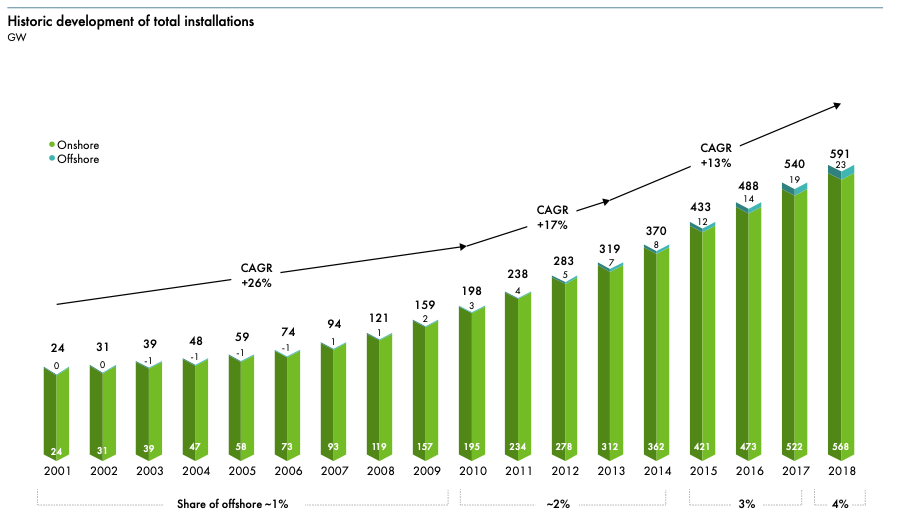
\includegraphics[width=1\textwidth]{风电装机容量历史变化}
    \bicaption{风电装机容量历史变化。来源:\href{https://www.ren21.net/wp-content/uploads/2019/05/gsr_2019_full_report_en.pdf}{REN21 2019 global status report}。}{Historical evolution of wind energy capacity. Source: \href{https://www.ren21.net/wp-content/uploads/2019/05/gsr_2019_full_report_en.pdf}{REN21 2019 global status report}}
    \label{fig:windcapacityhistory}
\end{figure}

鉴于全球风电市场的规模和影响力,相关研究也不断涌现。\citet{archer2005evaluation}利用全球陆地和探空观测差值到80 $m$(商用发电机高度在80-120 $m$)计算得到全球约13\%的站点年均风速大于6.9 $m ~ s^{-1}$(风电3类风力及以上,适合建设风电场),其中美国中部地区,欧洲北海沿岸地区此类站点较为集中。如果将此类站点所在区域都建设风电场,那么以2000年的情况,假设风力发电机能够捕获20\%的风能,那么风电发电量可以满足全球所有能源需求(约全球用电量的7倍)。\citet{lu2009global}利用GEOS-5同化全球各种观测资料得到的格点风场资料(水平分辨率67 $\times$ 50 $km$,垂直最低两层的高度约为71 $m$和201 $m$)差值到100 $m$计算全球陆地风能资源。若去除掉不适合建设风电场的城市、森林、冰川,其他地区全部建设风电场,假设风电场的效率为20\%,那么以2006年的情况计算,风电发电量可以超过全球所有能源需求的5倍(全球用电量的40倍)。

然而,前人对于风能资源的诸多研究中几乎没有研究涉及它的历史长期变化。由第\ref{chap:SpatiotemporalCharacteristics}章可以知道,全球特别是北半球陆地地表风速出现了普遍减小,根据风能公式(第\ref{chap:intro}章公式 \ref{eq:windpower})),风速的变化会在风能密度中被放大,因而风能资源在近十年来应当也出现了减少,但目前没有研究对这种影响进行定量估计。本章将首先评估近几十年来陆地风能资源的整体状况,然后分析风速长期变化对于风能资源的影响。

此外,目前对于风能资源未来变化的研究高度依赖全球气候模式\citep{pryor2011assessing, karnauskas2018southward},而以往对于全球气候模式对风能模拟能力的评估也几乎都没有考察其历史长期变化,这会大大影响研究者对于全球气候模式预估结果不确定性的估计。本章将评估全球气候模式对风能历史长期变化的模拟能力。

\section{资料和方法}

本章使用了NCEI-CMDC风速资料和ERA-Interim再分数据集6小时分辨率10 $m$ U、V风场数据用于风能资源估计,数据相关介绍见第\ref{chap:SpatiotemporalCharacteristics}章。

陆地地表风速模拟数据来自CMIP5的34个全球气候模式,模式简介见表 \ref{tab:descriptionGCM}。本章使用了包含自然和人为强迫的历史模拟月平均数据。值得一提的是CSIRO-MK3.6地表风速的高度是2 $m$,而所有其他模式都是10 $m$。

\begin{table}[!htbp]
    \bicaption{全球气候模式信息}{Description of global climate models}
    \label{tab:descriptionGCM}
    \centering
    \small% fontsize
    \setlength{\tabcolsep}{7 pt}% column separation
    \renewcommand{\arraystretch}{1.0}%row space 
    \begin{tabular}{llll}
        \hline
         模式名称 & 开发机构(所在国家) & 大气模式水平分辨率 & 参考文献 \\
        %\cline{2-9}% partial hline from column i to column j
        \hline
        ACCESS1.0 & CSIRO-BOM (澳大利亚) & 1.875$^\circ ~ \times$  1.25$^\circ$ & \citet{dix2013the} \\
        ACCESS1.3 & CSIRO-BOM (澳大利亚) & 1.875$^\circ ~ \times$  1.25$^\circ$ & \citet{dix2013the} \\
        BCC-CSM1.1 & BCC-CMA(中国) & 2.8 $^\circ ~ \times$ 2.8$^\circ$ & \citet{xin2013climate} \\
        BCC-CSM1.1(m) & BCC-CMA(中国) & 160 $\times$ 320 T106 & \citet{liu2015performance} \\
        BNU-ESM & GCESS(中国)& 2.8$^\circ ~ \times$ 2.8$^\circ$  & \citet{ji2014description} \\
        CanESM2 & CCCMA(加拿大) & 2.8$^\circ ~ \times$ 2.8$^\circ$ & \citet{arora2011carbon} \\
        CMCC-CESM & CMCC(意大利) & 3.75$^\circ ~ \times$ 3.75$^\circ$ & \citet{Fogli2009INGV} \\
        CMCC-CM & CMCC(意大利) & 0.75$^\circ ~ \times$ 0.75$^\circ$ & \citet{Fogli2009INGV} \\
        CMCC-CMS & CMCC(意大利)& 1.875$^\circ ~ \times$ 1.875$^\circ$ & \citet{Fogli2009INGV} \\
        CSIRO-Mk3.6.0 & CSIRO-QCCC(澳大利亚)& 1.875$^\circ ~ \times$ 1.875$^\circ$ & \citet{gordon2002csiro} \\
        FGOALS-s2 & LASG-IAP-CAS(中国)& 2.81$^\circ ~ \times$ 1.66$^\circ$ & \citet{bao2013flexible} \\
        GFDL-CM3 & NOAA GFDL(美国) & 1.875$^\circ ~ \times$ 1.875$^\circ$ & \citet{griffies2011gfdl} \\
        GFDL-ESM2G & NOAA GFDL(美国)& 2.5$^\circ ~ \times$ 2$^\circ$ & \citet{dunne2012gfdl,dunne2013gfdl} \\
        GFDL-ESM2M & NOAA GFDL(美国)& 2.5$^\circ ~ \times$ 2$^\circ$ & \citet{dunne2012gfdl,dunne2013gfdl} \\
        GISS-E2-H & NASA GISS(美国)& 2.5$^\circ ~ \times$ 2$^\circ$ & \citet{schmidt2014configuration} \\       
        \hline
	\end{tabular}
\end{table}
\begin{table}[!t]
    \ContinuedFloat% continue splited float
    \bicaption{续表。}{Continued table.}
    \label{tab:descriptionGCM2}
    \centering
    \small% fontsize
    \setlength{\tabcolsep}{7 pt}% column separation
    \renewcommand{\arraystretch}{1.0}%row space  
     \begin{tabular}{llll}
        \hline 
        GISS-E2-H-CC &  NASA GISS(美国)& 1$^\circ ~ \times$ 1$^\circ$ & \citet{schmidt2014configuration} \\
        GISS-E2-R & NASA GISS(美国) & 2.5$^\circ ~ \times$ 2$^\circ$ & \citet{schmidt2014configuration} \\
        GISS-E2-R-CC & NASA GISS(美国)& 1$^\circ ~ \times$ 1$^\circ$ & \citet{schmidt2014configuration} \\
        HadCM3 & MOHC(英国)& 3.75$^\circ ~ \times$ 2.5$^\circ$ & \citet{johns2003anthropogenic} \\
        HadGEM2-AO & MOHC(英国)& 1.875$^\circ ~ \times$ 1.25$^\circ$ & \citet{collins2011development} \\
        HadGEM2-CC & MOHC(英国)& 1.875$^\circ ~ \times$ 1.25$^\circ$ & \citet{collins2011development} \\
        HadGEM2-ES & MOHC(英国)& 1.875$^\circ ~ \times$ 1.25$^\circ$ & \citet{collins2011development} \\
        INM-CM4 & INM(俄罗斯)& 2$^\circ ~ \times$ 1.5$^\circ$ & \citet{volodin2010simulating} \\
        IPSL-CM5A-LR & IPSL(法国)& 3.75$^\circ ~ \times$ 1.9$^\circ$ & \citet{dufresne2013climate} \\
        IPSL-CM5A-MR &  IPSL(法国)& 2.5$^\circ ~ \times$ 1.25$^\circ$ & \citet{dufresne2013climate} \\
        IPSL-CM5B-LR & IPSL(法国)& 3.75$^\circ ~ \times$ 1.9$^\circ$ & \citet{dufresne2013climate} \\
        MIROC4h & MIROC(日本)& 0.56$^\circ ~ \times$ 0.56$^\circ$ & \citet{sakamoto2012miroc4h} \\
        MIROC5 & MIROC(日本)& 1.4$^\circ ~ \times$ 1.4$^\circ$ & \citet{watanabe2010improved} \\
        MIROC-ESM & MIROC(日本)& 2.8$^\circ ~ \times$ 2.8$^\circ$ & \citet{watanabe2010improved} \\
        MIROC-ESM-CHEM & MIROC(日本)& 2.8$^\circ ~ \times$ 2.8$^\circ$ &  \citet{watanabe2010improved} \\
        MPI-ESM-LR & MPI-M(德国)& 1.8$^\circ ~ \times$ 1.8$^\circ$ & \citet{giorgetta2013climate} \\
        MPI-ESM-MR & MPI-M(德国)& 1.8$^\circ ~ \times$ 1.8$^\circ$ & \citet{giorgetta2013climate} \\
        MPI-ESM-P & MPI-M(德国)& 1.8$^\circ ~ \times$ 1.8$^\circ$ & \citet{giorgetta2013climate} \\
        MRI-CGCM3 & MRI(日本)& 320 $\times$ 160 T159 & \citet{yukimoto2012a} \\
        \hline
      \end{tabular}
\end{table}
    
由于风速观测取自于10 $m$附近,而风力发电机高度约为100 $m$,使用power law \citep{peterson1978on}将10 $m$风速差值到100 $m$:

\begin{equation} \label{eq:powerlaw}
\frac{U_{2}}{U_{1}} = \left( \frac{z_{2}}{z_{1}} \right)^{\alpha}
\end{equation} ~\\
其中$U_{2}$和$U_{1}$分别是$z_{2}$和$z_{1}$高度的风速,$\alpha$是一个经验参数,在大气稳定度为中性且周边较为平坦开阔的情况下,$\alpha$约为0.14。

通常认为,风速满足双参数Weibull分布 \citep{pryor2010climate},其概率密度分布函数(PDF)为:

\begin{equation} \label{eq:weibull}
f(x) = \frac{b}{a} \left( \frac{x}{a} \right)^{b-1} exp \left[-\left(\frac{x}{a} \right)^{b} \right]
\end{equation} ~\\
其中$a$为尺度参数,$b$为形状参数。估计$a$和$b$数值方法如下\citep{monahan2006the1,monahan2006the2}:

\begin{equation} \label{eq:weibullparameter}
b = \left(\frac{\bar{x}}{\sigma} \right)^{1.086}
\end{equation}  
\vspace*{1ex}  
\begin{equation} \label{eq:weibullparameter2}
a = \frac{\bar{x}}{\Gamma \left(1 + \frac{1}{b} \right)}
\end{equation} ~\\
其中,$\bar{x}$为样本均值,可使用观测值估计,$\sigma$为样本标准差,可使用ERA-Interim资料估计,因为NCEI-CMDC为日平均数据,而公式 \ref{eq:weibullparameter}最适用于原始观测数据,即由单次观测组成的观测资料,ERA-Interim 6小时分辨率风场资料与此类似。$\Gamma$为Gamma函数:

\begin{equation} \label{eq:gammafunction}
\Gamma(x) = \int_{0}^{\infty} t^{x - 1} e^{-t} dt 
\end{equation} ~\\
将(第\ref{chap:intro}章公式  \ref{eq:windpower})代入,得到:

\begin{equation} \label{eq:windpowerwithweibull}
E = \frac{1}{2} \rho a^{3} \Gamma \left( 1 + \frac{3}{b} \right)
\end{equation} ~\\
其中,$\rho$为空气密度,在15摄氏度标准大气压下为1.225 $kg ~ m^{-3}$。

\section{北半球风能资源评估}

由1979-2016年气候态风场计算北半球风能密度分布,计算时将风力发电机可利用的风速设定为3-25 $m ~ s^{-1}$,得到北半球中位数风能密度为118 $W ~ m^{-2}$,北美洲为183 $W ~ m^{-2}$,欧洲为181 $W ~ m^{-2}$,亚洲为46 $W ~ m^{-2}$,亚洲显著小于北美洲和欧洲。总体来看沿海地区风能密度大于内陆,北美洲除外,其风能密度最高的地区在中部地区(图 \ref{fig:NHwindpower})。下面逐个大洲进行分析。

\begin{figure}[!htbp]
    \centering
    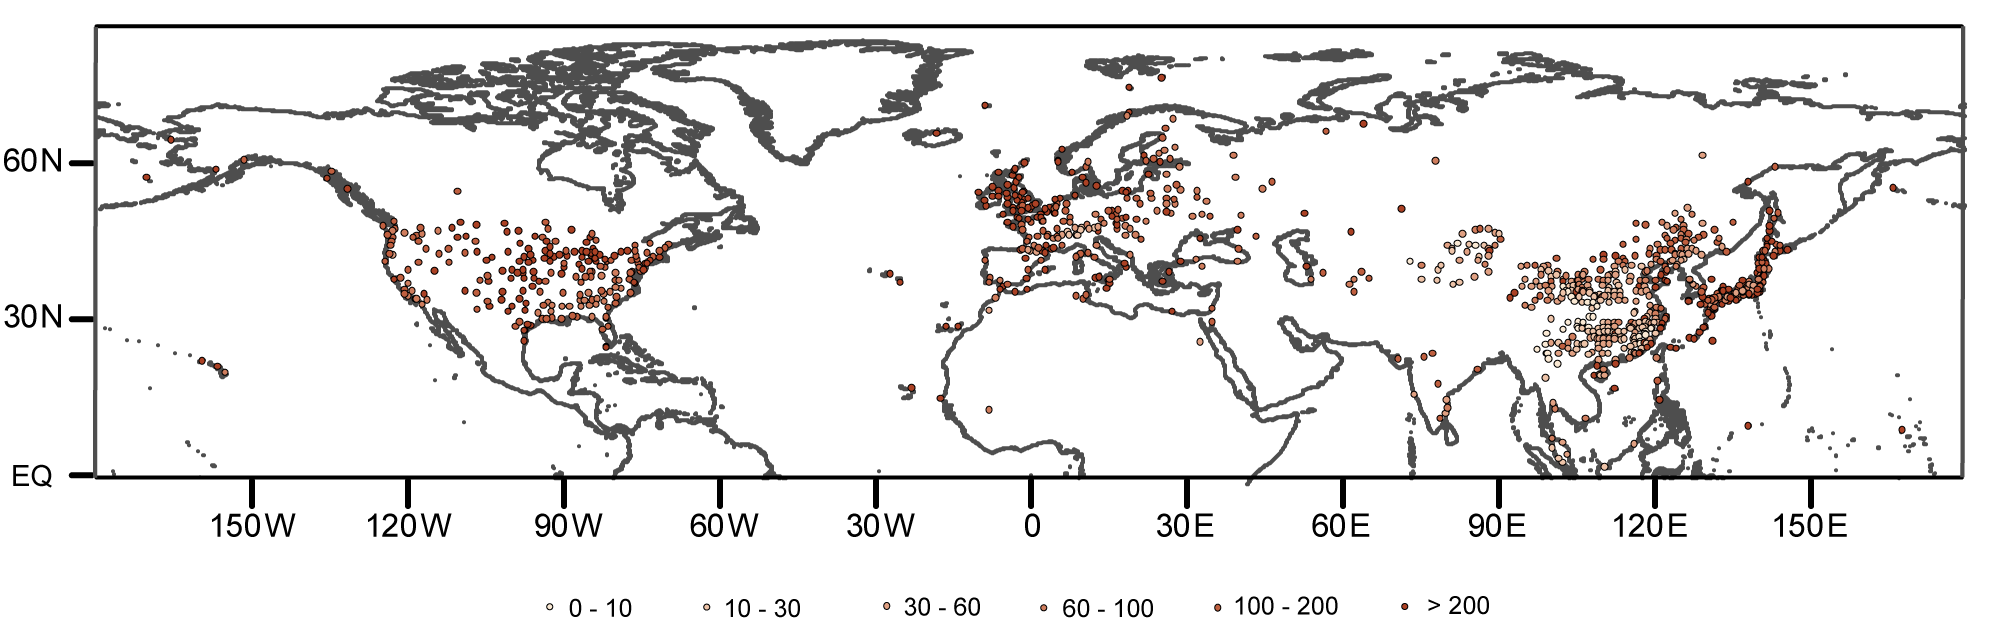
\includegraphics[width=1\textwidth]{北半球风能密度}
    \bicaption{北半球风能密度( $W ~ m^{-2}$)}{Wind power density in the Northern Hemisphere ( in $W ~ m^{-2}$) }
    \label{fig:NHwindpower}
\end{figure}

北美洲中部和东北部风能密度较大,多数站点超过200 $W ~ m^{-2}$,中部风能密度最大,大部分站点超过250 $W ~ m^{-2}$。相比之下,北美西海岸和东南部风能密度多在150 $W ~ m^{-2}$以下(图 \ref{fig:NAwindpower})。对比美国风力发电场分布,主要分布在中部和中西部地区,而东南部没有一座风电场,这与风能密度分布基本吻合。然而,西南部的加利福尼亚州也安装了大量风力发电机,占到全美总量的24\%,原因是加利福尼亚州经济发达且环保观念较强,加州甚至立法要求全州公用事业单位在2030年前要实现一半电力来自可再生能源(\href{https://www.energy.ca.gov/rules-and-regulations/energy-suppliers-reporting/clean-energy-and-pollution-reduction-act-sb-350}{《清洁能源和减少污染法案》 SB 350}),因而此地区有较强的使用风力发电的能力和愿望(图 \ref{fig:NAturbinelocation})。可见风电的分布不仅取决于风能资源情况,也受到地方经济发展水平和观念的影响。

\begin{figure}[!htb]
    \centering
    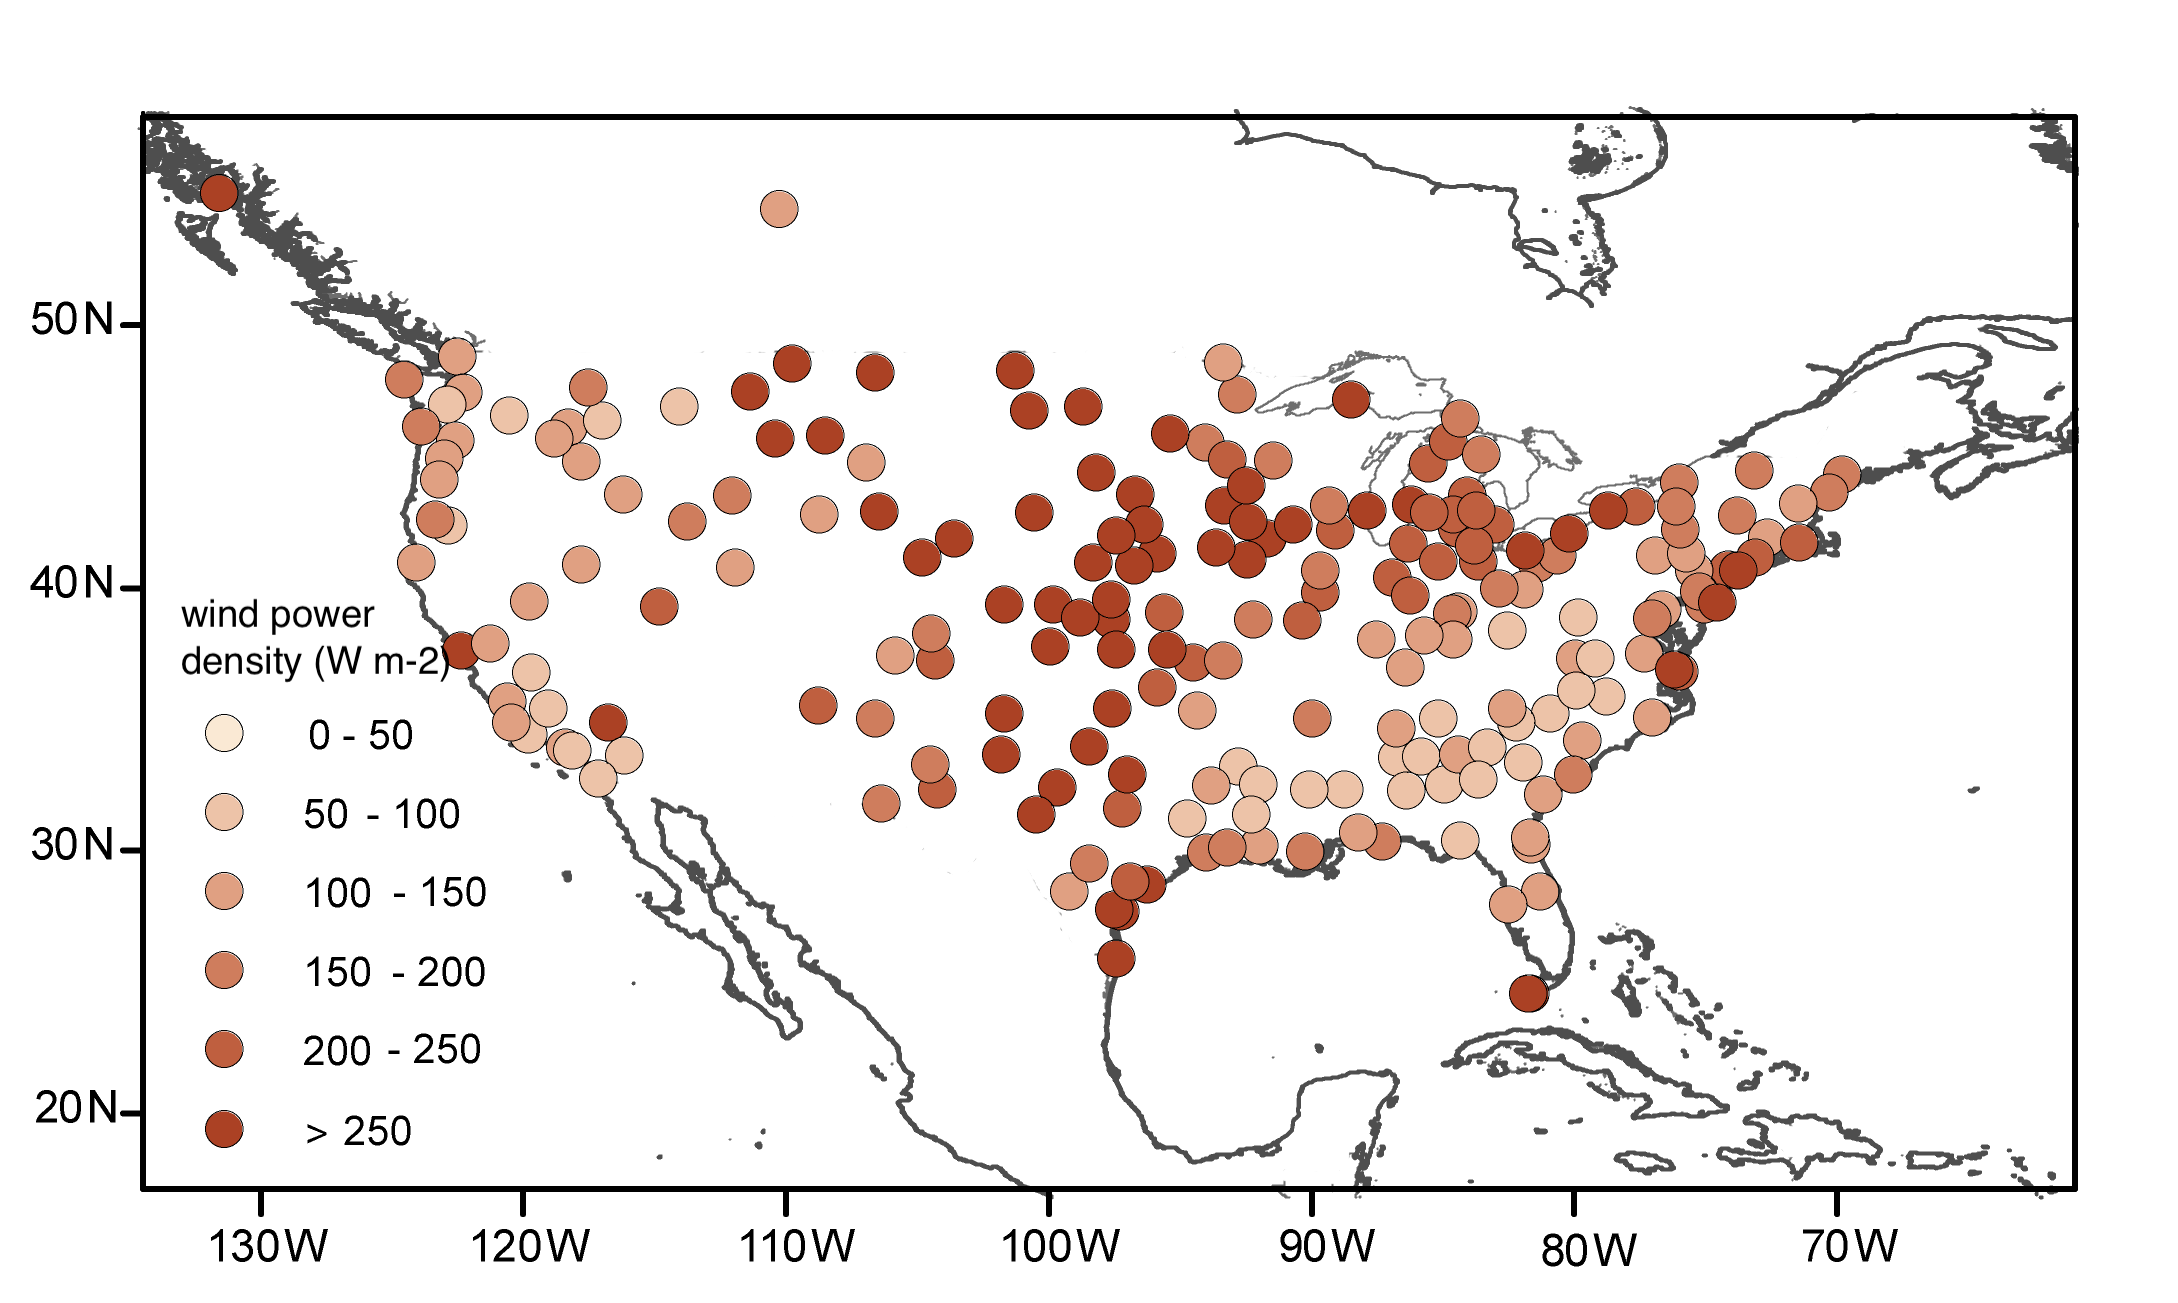
\includegraphics[width=0.8\textwidth]{北美风能密度}
    \bicaption{北美风能密度($ W ~ m^{-2}$)}{Wind power density in North America (in $ W ~ m^{-2}$)}
    \label{fig:NAwindpower}
\end{figure}

\begin{figure}[!htb]
    \centering
    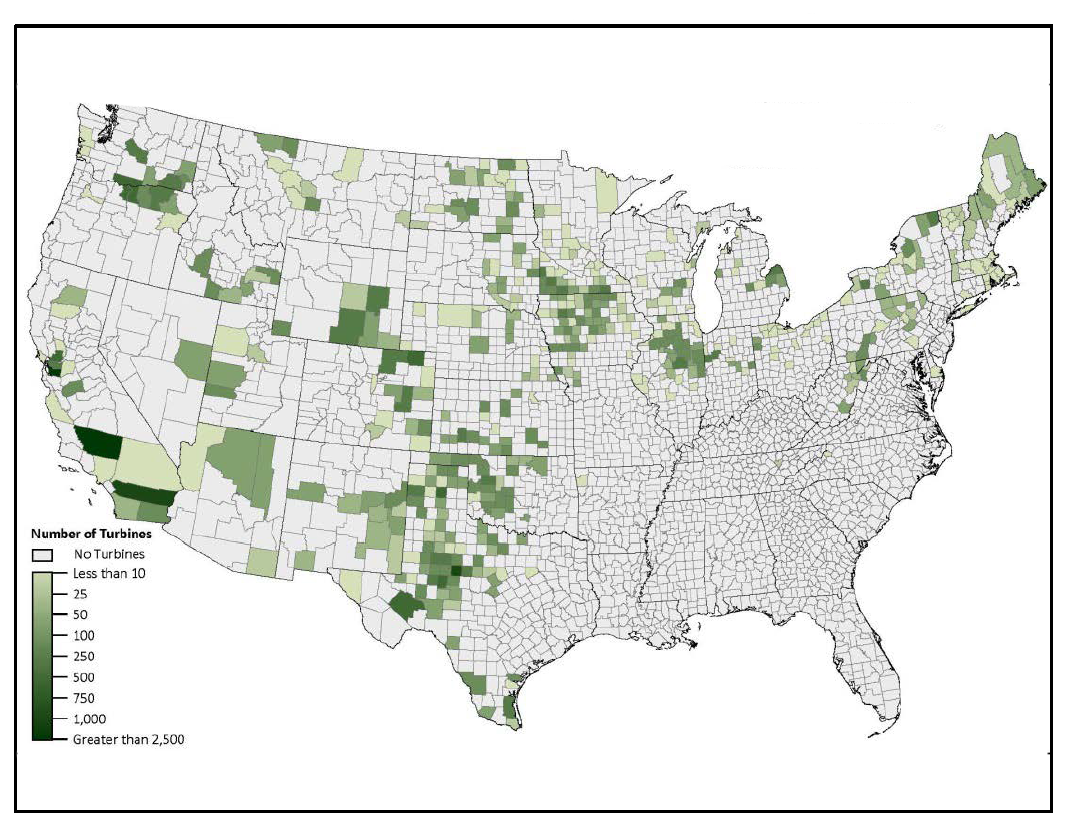
\includegraphics[width=0.75\textwidth]{美国风机分布}
    \bicaption{美国风机分布。来源:\href{https://www.usda.gov/oce/energy/files/FINAL-Wind_Energy_Land_Distribution_in_the_United_States_of_America_7282017.pdf}{Wind Energy Land Distribution In The United States of America}。}{North American wind turbine locations. Source: \href{https://www.usda.gov/oce/energy/files/FINAL-Wind_Energy_Land_Distribution_in_the_United_States_of_America_7282017.pdf}{Wind Energy Land Distribution In The United States of America}.}
    \label{fig:NAturbinelocation}
\end{figure}

欧洲风能密度最大的区域在北海沿岸,包括英国、法国和德国的沿海地区,风能密度大多在200 $W ~ m^{-2}$以上。相比之下,欧洲内陆地区风能密度普遍较低,大部分站点在150 $W ~ m^{-2}$以下(图 \ref{fig:EUwindpower})。欧洲风电场最密集的国家是德国,其次是英国和西班牙,其中英国是风电装机总量前十国家中海上风电占比最高的,达到1/3。法国,瑞典和意大利也有大量的风电场运行(图 \ref{fig:EUturbinelocation})。对比风能资源与风电场的分布,发现风电场主要分布在风能资源丰富的地区。值得一提的是,由于德国长时间地面观测资料较为缺乏,在研究中缺少其风能资源状况的数据,但根据\citet{lu2009global}使用2006年风场测算,德国沿海地区风能资源非常丰富(与法国类似),十分适合风力发电。此外,德国的雄厚工业实力以及强烈的环保观念也起到了很大影响,德国拥有西门子、Enercon、Repower等一批风机制造领域有影响力的公司,德国也于2000年通过《可再生能源法》(\href{https://www.lexadin.nl/wlg/legis/nofr/eur/arch/ger/resact.pdf}{EEG-2000})对于可再生能源行业进行扶持。

\begin{figure}[!htbp]
    \centering
    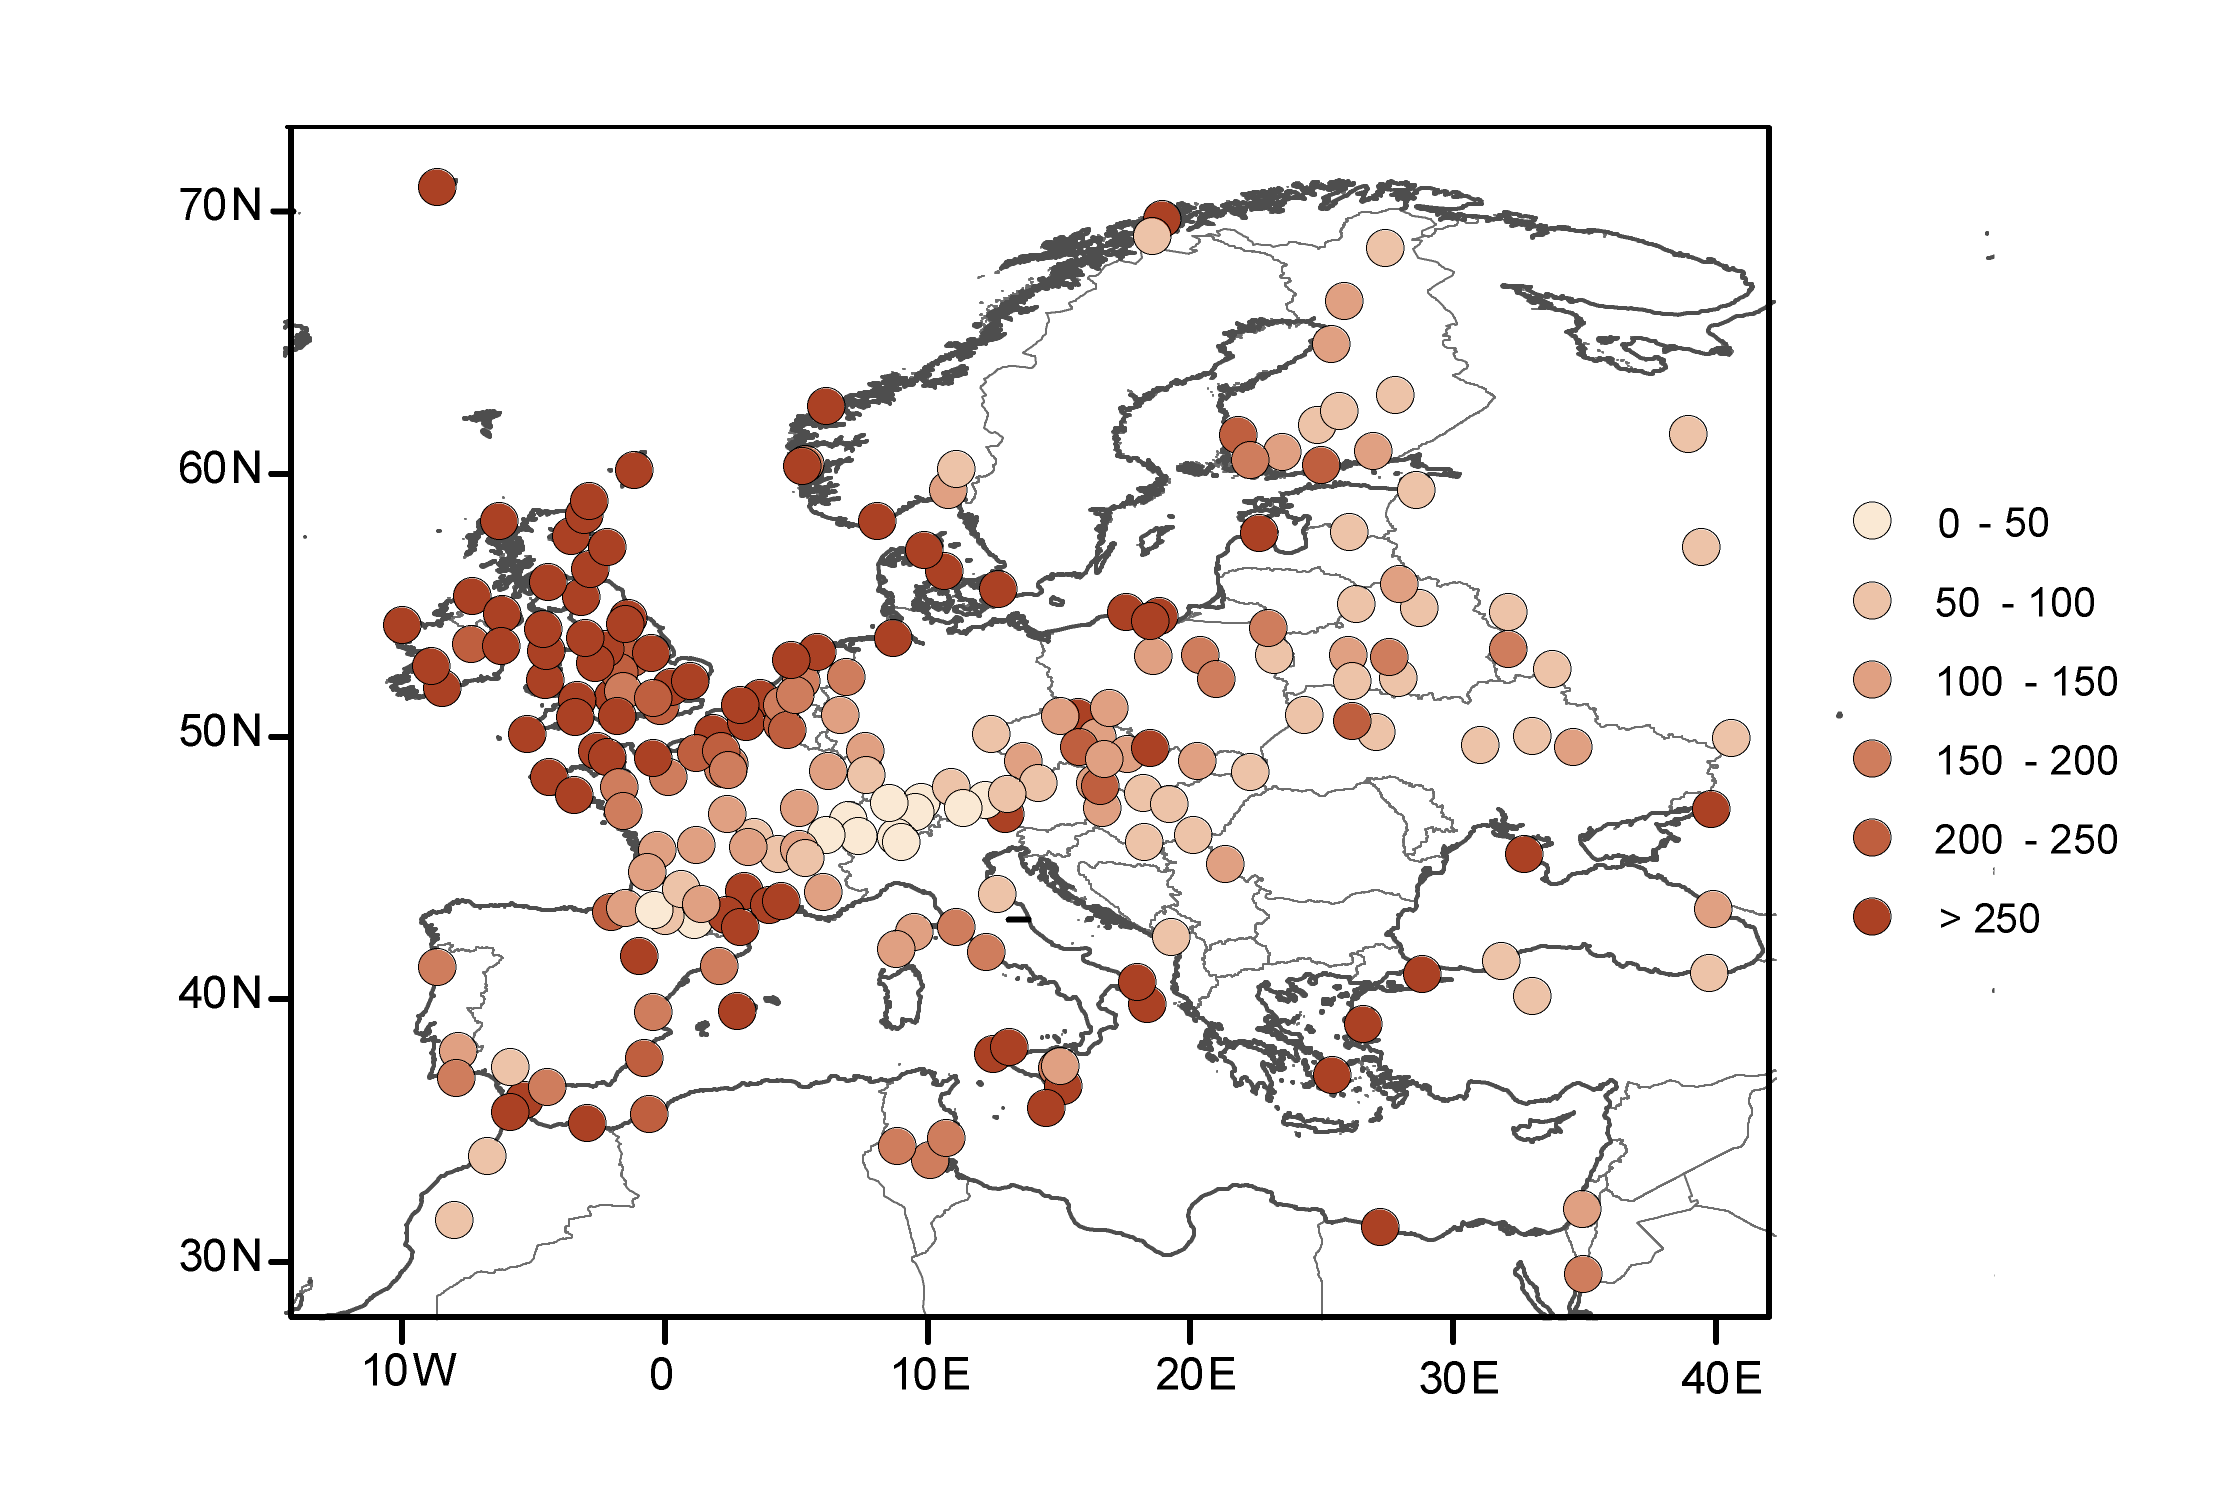
\includegraphics[width=0.95\textwidth]{欧洲风能密度}
    \bicaption{欧洲风能密度($ W ~ m^{-2}$)}{Wind power density in Europe (in $ W ~ m^{-2}$)}
    \label{fig:EUwindpower}
\end{figure}

\begin{figure}[!htbp]
    \centering
    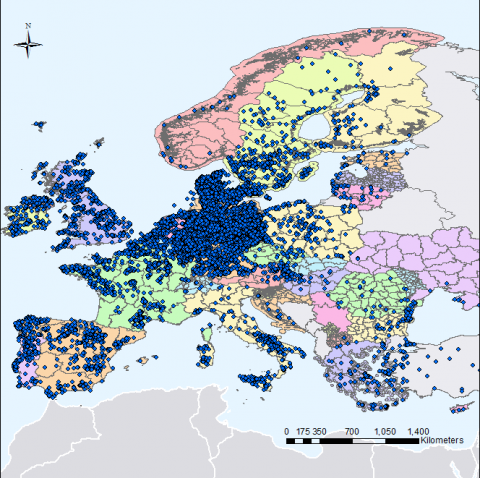
\includegraphics[width=0.65\textwidth]{欧洲风机分布}
    \bicaption{欧洲风机分布。来源:\href{https://setis.ec.europa.eu/sites/default/files/reports/emhires_dataset_part_i_wind_power_generation_0.pdf}{EMHIRES dataset
Part I: Wind power generation}。}{European wind turbine locations. Source: \href{https://setis.ec.europa.eu/sites/default/files/reports/emhires_dataset_part_i_wind_power_generation_0.pdf}{EMHIRES dataset
Part I: Wind power generation}.}
    \label{fig:EUturbinelocation}
\end{figure}

亚洲多数站点分布在中国和日本,其中日本沿海地区风能资源较为丰富,中国沿海地区同样是风能资源较为丰富的地区,除沿海外,中国东北和内蒙古中部地区也有较为丰富的风能资源,多在100 $W ~ m^{-2}$以上(图 \ref{fig:ASwindpower})。由于日本风电产业并不发达,装机容量仅为中国的1/70,因而这里不对日本风电场分布进行分析。中国在全球风电行业处于领先位置并在近年来一直保持高速增长,目前风电场集中分布于东部沿海地区,黑龙江、河北,内蒙古中部、甘肃酒泉和新疆哈密等地区,其中,内蒙古在各省中装机容量排名第一,其后是新疆、甘肃和河北(图 \ref{fig:CHNturbinelocation})。中国风电场的分布与风能密度高的地区高度重合,表明风电场规划选址十分科学合理。中国风电产业的发展主要依赖于政策的扶持,中国政府出台了一系列优惠政策鼓励风电产业发展,包括对银行贷款给予财政补贴,增值税优惠,设备进口关税优惠和对风电相关技术研究的资助等(\href{http://www.nea.gov.cn/2017-11/02/c_136722869.htm}{《中华人民共和国可再生能源法》})。

\begin{figure}[!htbp]
    \centering
    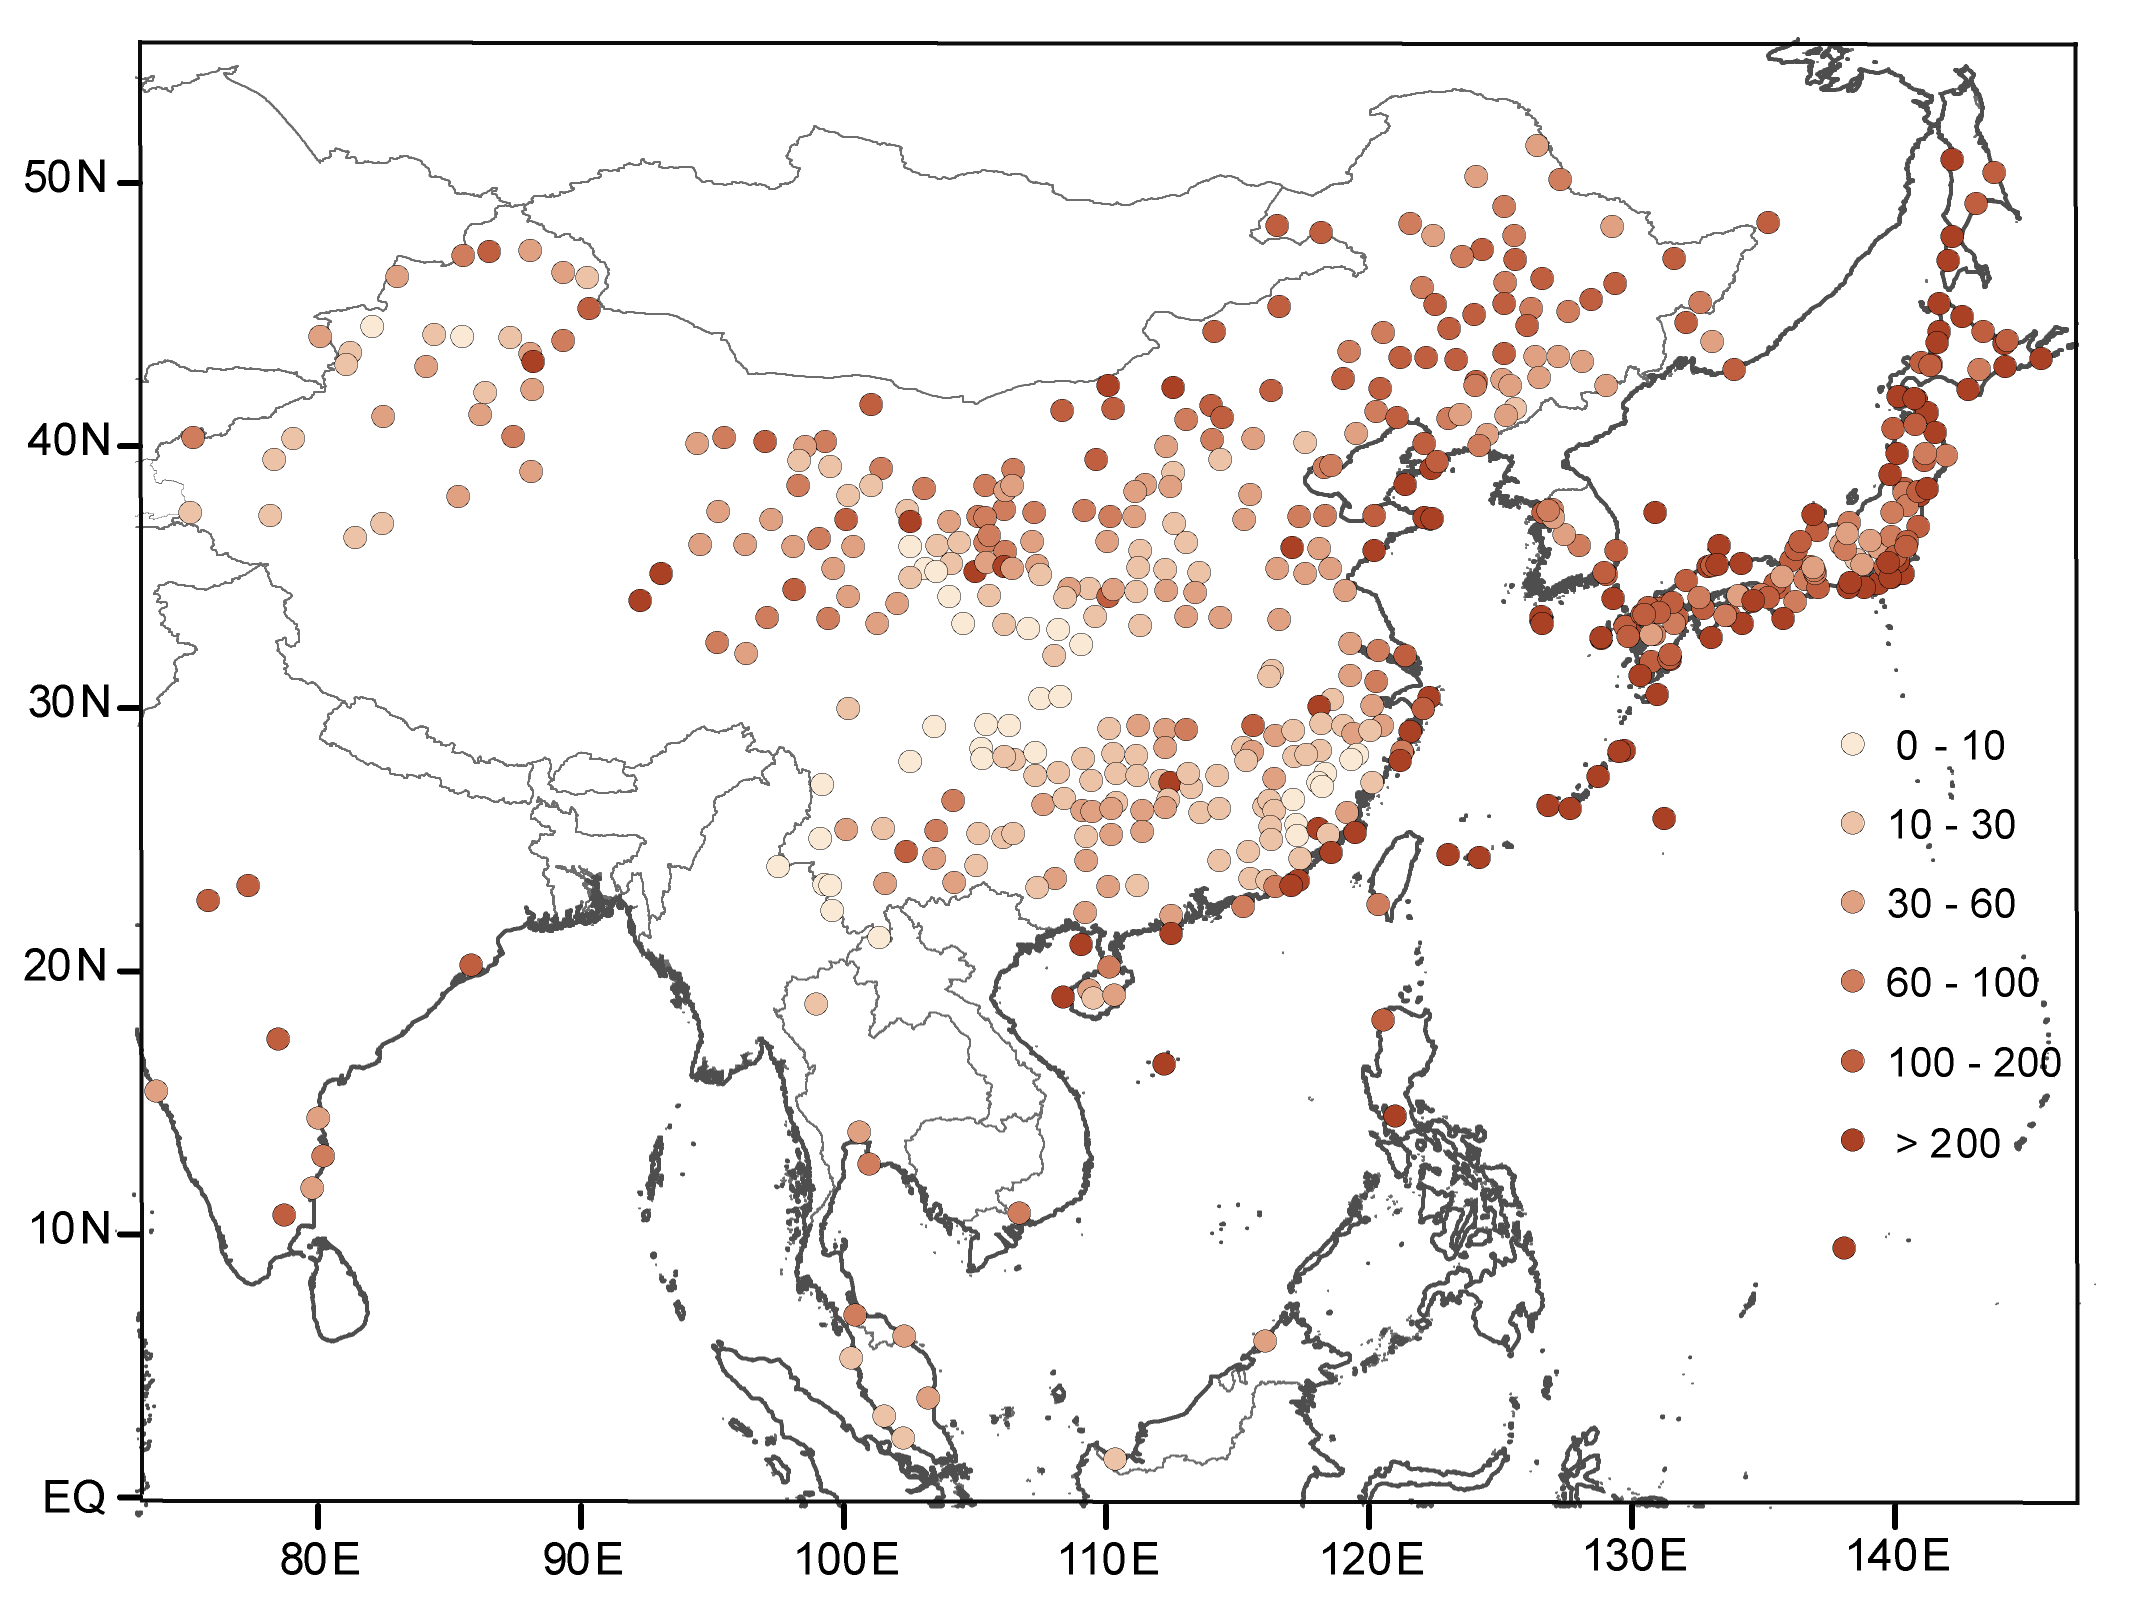
\includegraphics[width=0.85\textwidth]{亚洲风能密度}
    \bicaption{亚洲风能密度($ W ~ m^{-2}$)}{Wind power density in Asia (in $ W ~ m^{-2}$)}
    \label{fig:ASwindpower}
\end{figure}

\section{陆地地表风速长期变化对风能资源的影响}

1979年至今,受到地表风速普遍减小的影响,北半球风能密度也出现了显著减小,中位数风能密度从1979年的132 $W ~ m^{-2}$到2016年的108 $W ~ m^{-2}$。在2007年前风能密度减小迅速,而其后风能密度有微弱下降,这与风速变化基本一致,表明风能密度变化由平均风速变化主导(图 \ref{fig:NHwindpowerevolution})。用2012-2016年平均风能密度减去1979-2003年平均风能密度得到风能密度变化的空间分布,发现北半球由75\%的站点风能密度下降,有8\%站点下降超过100 $W ~ m^{-2}$,1.5\%站点下降超过200 $W ~ m^{-2}$(图 \ref{fig:NHwindpowerchange} a));同时,也有5\%的站点上升超过50 $W ~ m^{-2}$,1.5\%站点上升超过100 $W ~ m^{-2}$。将风能密度变化除以1979-2003平均风能密度得到归一化风能密度变化,得到北半球风能密度变化的中位数为-14.8\%,有43\%站点减小超过20\%,15\%站点减小超过50\%;同时有15\%站点增长超过10\%,9\%站点增长超过20\%(图 \ref{fig:NHwindpowerchange} b))。下面各个大洲分别进行分析。

\begin{figure}[!t]
    \centering
    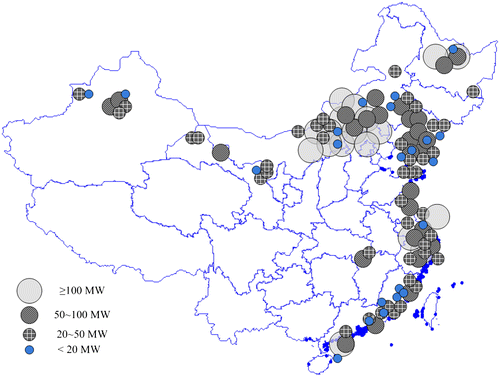
\includegraphics[width=0.7\textwidth]{中国风机分布}
    \bicaption{中国风电场分布及装机容量。来源:\citet{wang2011cost}。}{Chinese wind turbine locations. Source: \citet{wang2011cost}.}
    \label{fig:CHNturbinelocation}
\end{figure}

\begin{figure}[!b]
    \centering
    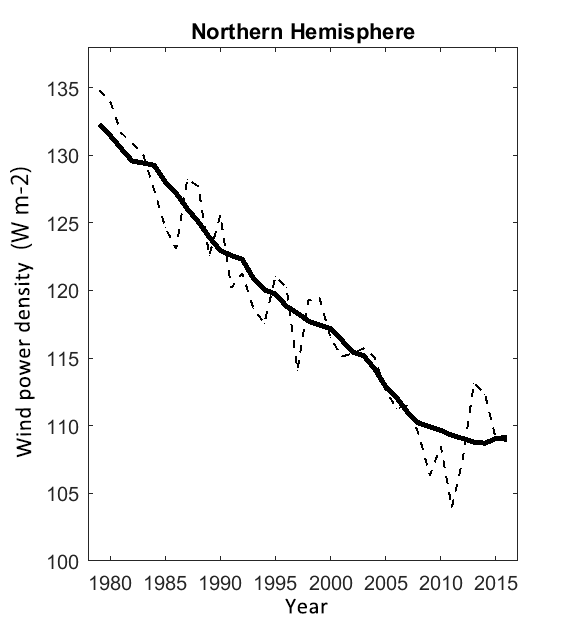
\includegraphics[width=0.45\textwidth]{北半球风能密度演变}
    \bicaption{北半球中位数风能密度演变($ W ~ m^{-2}$)。虚线为年平均值,实线为年平均值9点平滑后结果。}{Median wind power density evolution over the Northern Hemisphere (in $ W ~ m^{-2}$). Dash line is annual mean value, solid line is 9-point moving mean of dash line.}
    \label{fig:NHwindpowerevolution}
\end{figure}

\setupctable{captionsleft}% 标题朝向
\begin{sidewaysfigure}[!htbp]
    \centering
     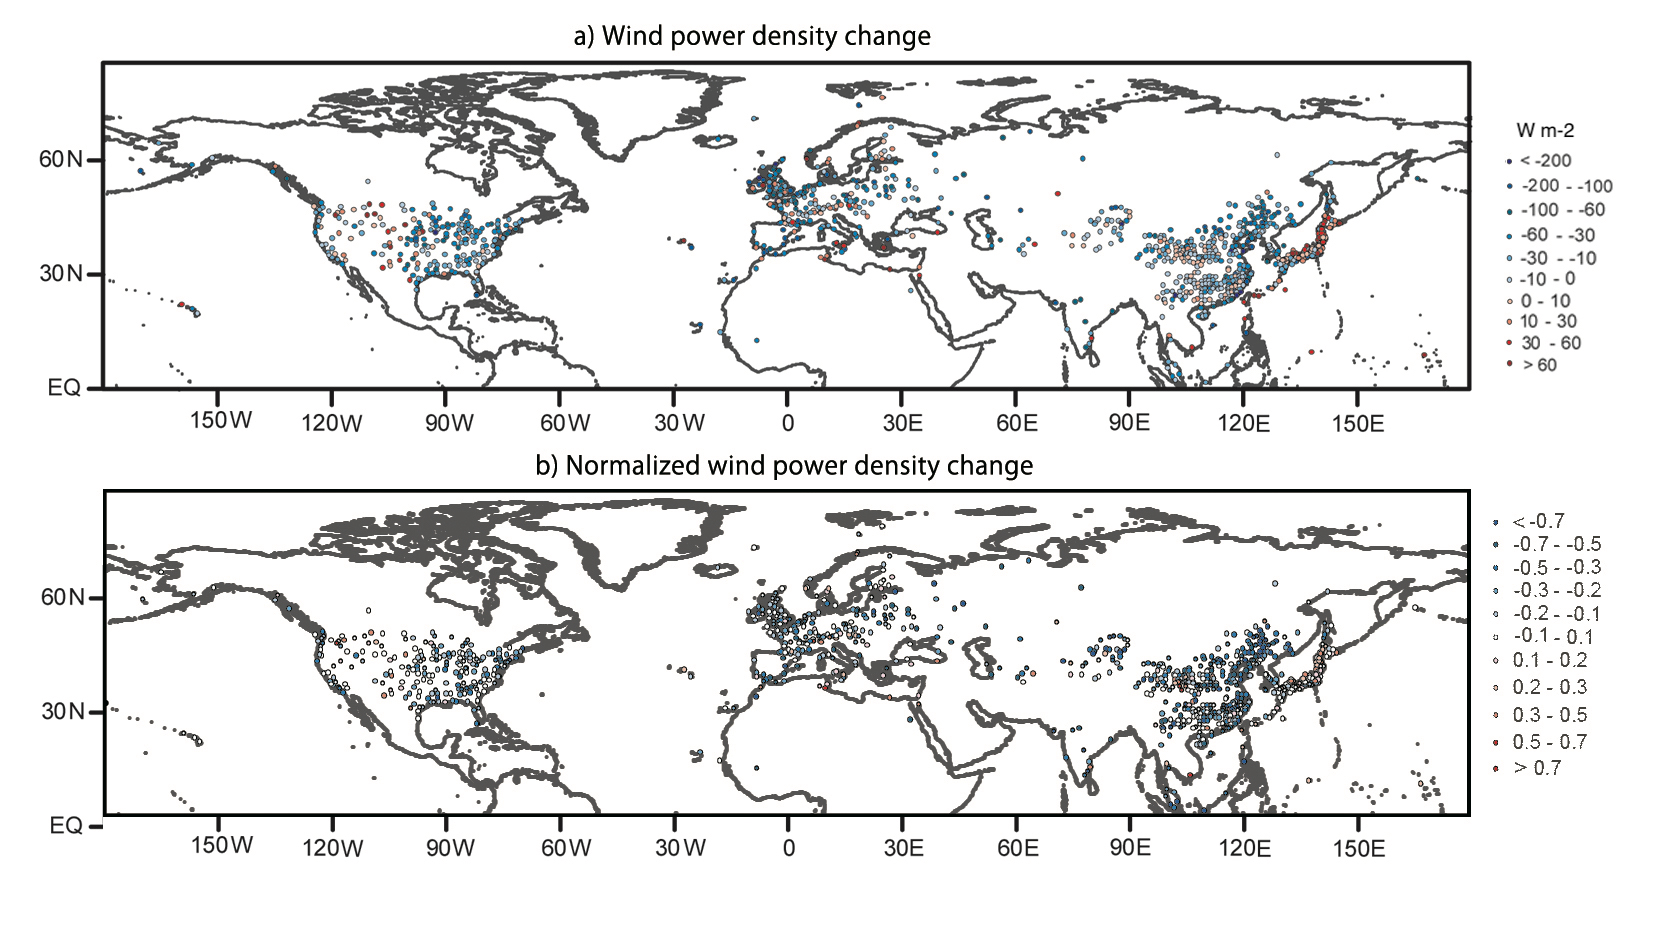
\includegraphics[width=1\textwidth]{北半球风能密度变化}
    \bicaption{北半球风能密度变化。a) 风能密度变化($W ~ m^{-2}$),b)归一化风能密度变化。}{Change in wind power density over the Northern Hemisphere. a) Wind power density change (in $ W ~ m^{-2}$), b) Normalized wind power density change.}
    \label{fig:NHwindpowerchange}
\end{sidewaysfigure}

北美洲214个站点风能密度变化中位数为-12.2\%,有30\%站点减小超过20\%,5\%站点减小超过50\%,另有11\%增加超过10\%,6\%站点增加超过20\%。风能密度减小明显的站点主要分布在东部地区和西海岸一线(图 \ref{fig:NAwindpowerchange})。在风力超过3类(平均风能密度100 m高度平均风能密度370 $W ~ m^{-2}$以上,适于建设风电场)的22个站点集中在中部带,其中风能密度变化中位数-16.7\%,其中有50\%的站点风能密度下降超过10\%,32\%的站点风能密度下降超过20\%,1个站点(4.5\%)风能密度下降超过50\%,另有1个站点风能密度增加超过10\%(图 \ref{fig:NAwindpowerchangeover3})。北美洲中位数风能密度在1993年前稳定在190 $W ~ m^{-2}$左右,1993-2007年有190 $W ~ m^{-2}$迅速下降至168 $W ~ m^{-2}$,趋势为-15.7 $W ~ m^{-2}$每十年,之后稳定在168 $W ~ m^{-2}$附近。而3类风力以上站点中位数风能密度1986年前在420 $W ~ m^{-2}$左右,之后在1986-1996年间迅速下降至380 $W ~ m^{-2}$,期间变化趋势为-40 $W ~ m^{-2}$每十年,1996-2008年下降速度趋缓,为-21 $W ~ m^{-2}$每十年,之后稳定在355 $W ~ m^{-2}$左右(图 \ref{fig:NAwindpowerevolution})。

\begin{figure}[!htbp]
    \centering
     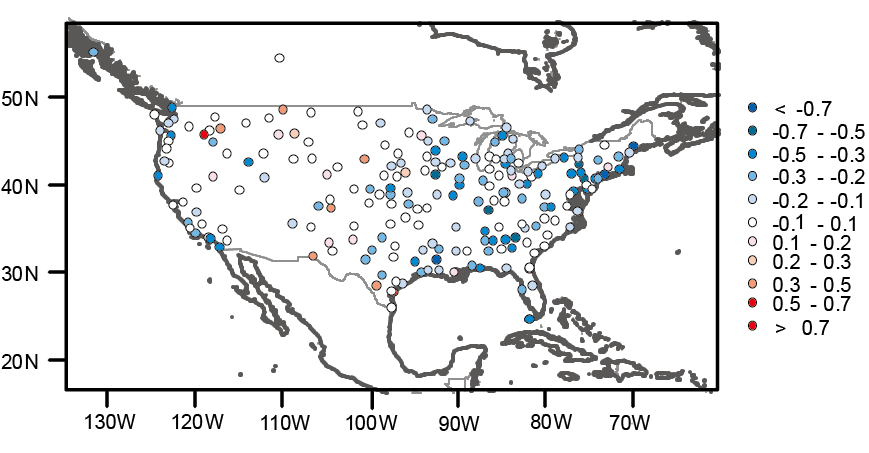
\includegraphics[width=1\textwidth]{北美风能密度变化}
    \bicaption{北美洲风能密度变化(变化率)}{Change in wind power density over North America (in $changing ~ rate$)}
    \label{fig:NAwindpowerchange}
\end{figure}

\begin{figure}[!htbp]
    \centering
     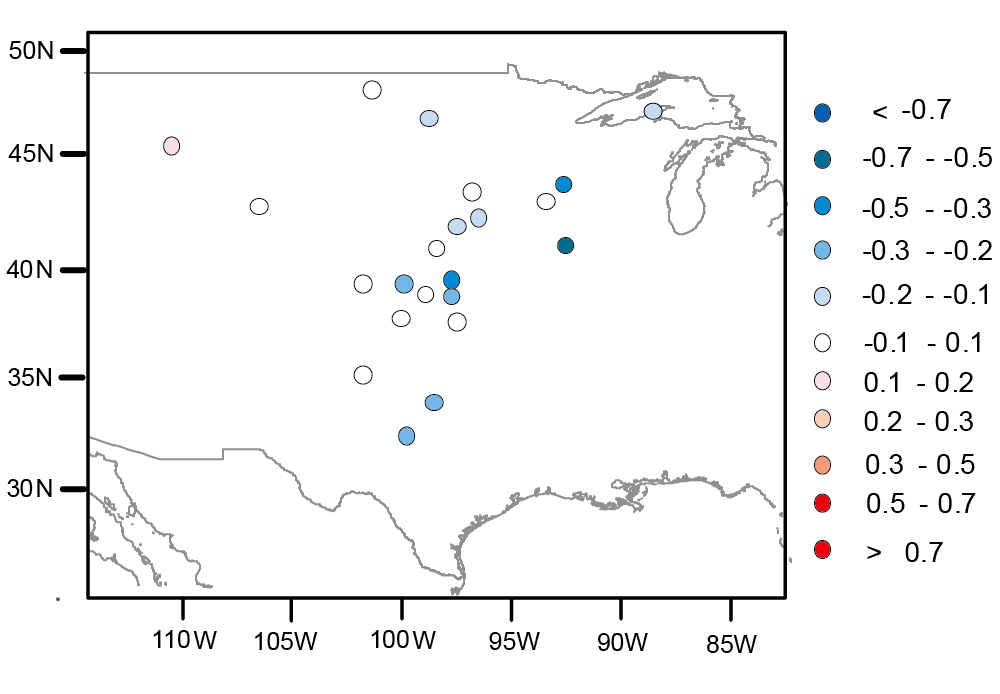
\includegraphics[width=0.9\textwidth]{北美大于3类风力站点风能密度变化}
    \bicaption{北美大于3类风力站点风能密度变化 (变化率)}{Change in wind power density at stations exceeding wind class 3 over North America (in $changing ~ rate$)}
    \label{fig:NAwindpowerchangeover3}
\end{figure}

\begin{figure}[!htbp]
    \centering
     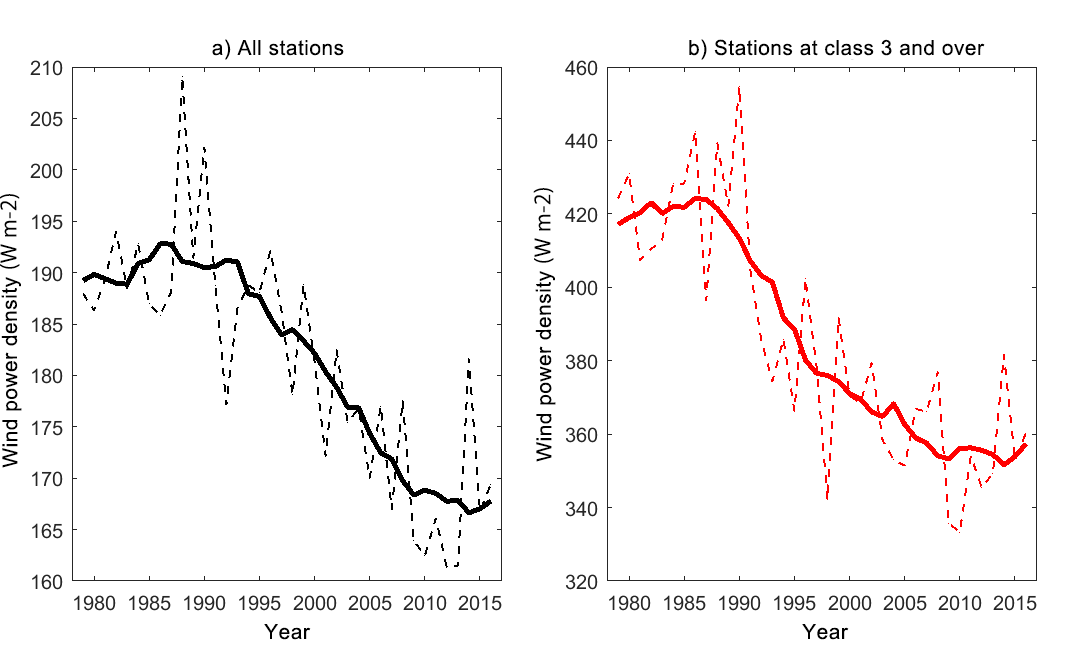
\includegraphics[width=0.9\textwidth]{北美洲风能密度演变}
    \bicaption{北美洲风能密度演变($ W ~ m^{-2}$)。a)所有站点中位数风能密度演变,b)超过3类风力站点中位数风能密度演变。虚线为年平均值,实线为年平均值9点平滑后结果。}{Change in wind power density over North America (in $ W ~ m^{-2}$). a)Median wind power density of all stations, b)Median wind power density of stations exceeding wind class 3. Dash line is annual mean value, solid line is 9-point moving mean of dash line.}
    \label{fig:NAwindpowerevolution}
\end{figure}

欧洲224个站点风能密度变化中位数为-15.2\%,有42\%站点减小超过20\%,15\%站点减小超过50\%,另外有16\%的站点增加超过10\%,8\%站点增加超过20\%。空间分布上,风能密度变化较为均匀(图 \ref{fig:EUwindpowerchange})。欧洲风力超过3类的站点有50个,主要分布在英国和欧洲大陆北海沿岸地区,另外在意大利南部、西班牙也有分布。这些站点风能密度变化中位数为-18\%,有72\%站点风能密度下降超过10\%,44\%的站点下降超过20\%,8\%站点下降超过50\%;另外有3个站点(6\%)风速增加超过10\%,仅有1个站点(2\%)风速增加超过20\%(图 \ref{fig:EUwindpowerchangeover3})。欧洲中位数风能密度从1979年的200 $W ~ m^{-2}$一路下降到2016年的162 $W ~ m^{-2}$,趋势为-10.5 $W ~ m^{-2}$每十年,超过3类风力在1990年前以-30 $W ~ m^{-2}$每十年的趋势下降,之后加速下降,在1990-2000年间趋势为-60 $W ~ m^{-2}$每十年,2000年后风能密度有缓慢上升,趋势为10 $W ~ m^{-2}$每十年(图 \ref{fig:EUwindpowerevolution})。

\begin{figure}[!htbp]
    \centering
     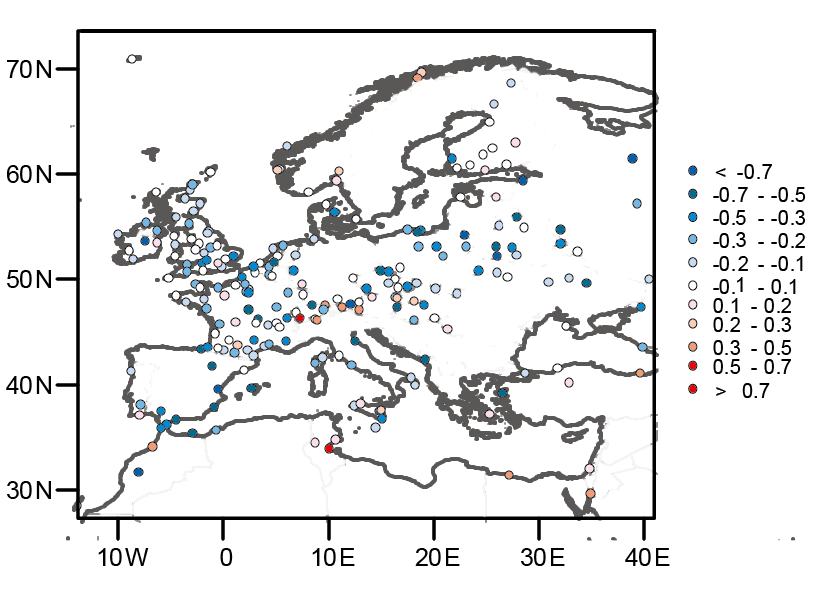
\includegraphics[width=0.9\textwidth]{欧洲风能密度变化}
    \bicaption{欧洲风能密度变化(变化率)}{Change in wind power density over Europe (in $changing ~ rate$)}
    \label{fig:EUwindpowerchange}
\end{figure}

\begin{figure}[!htbp]
    \centering
     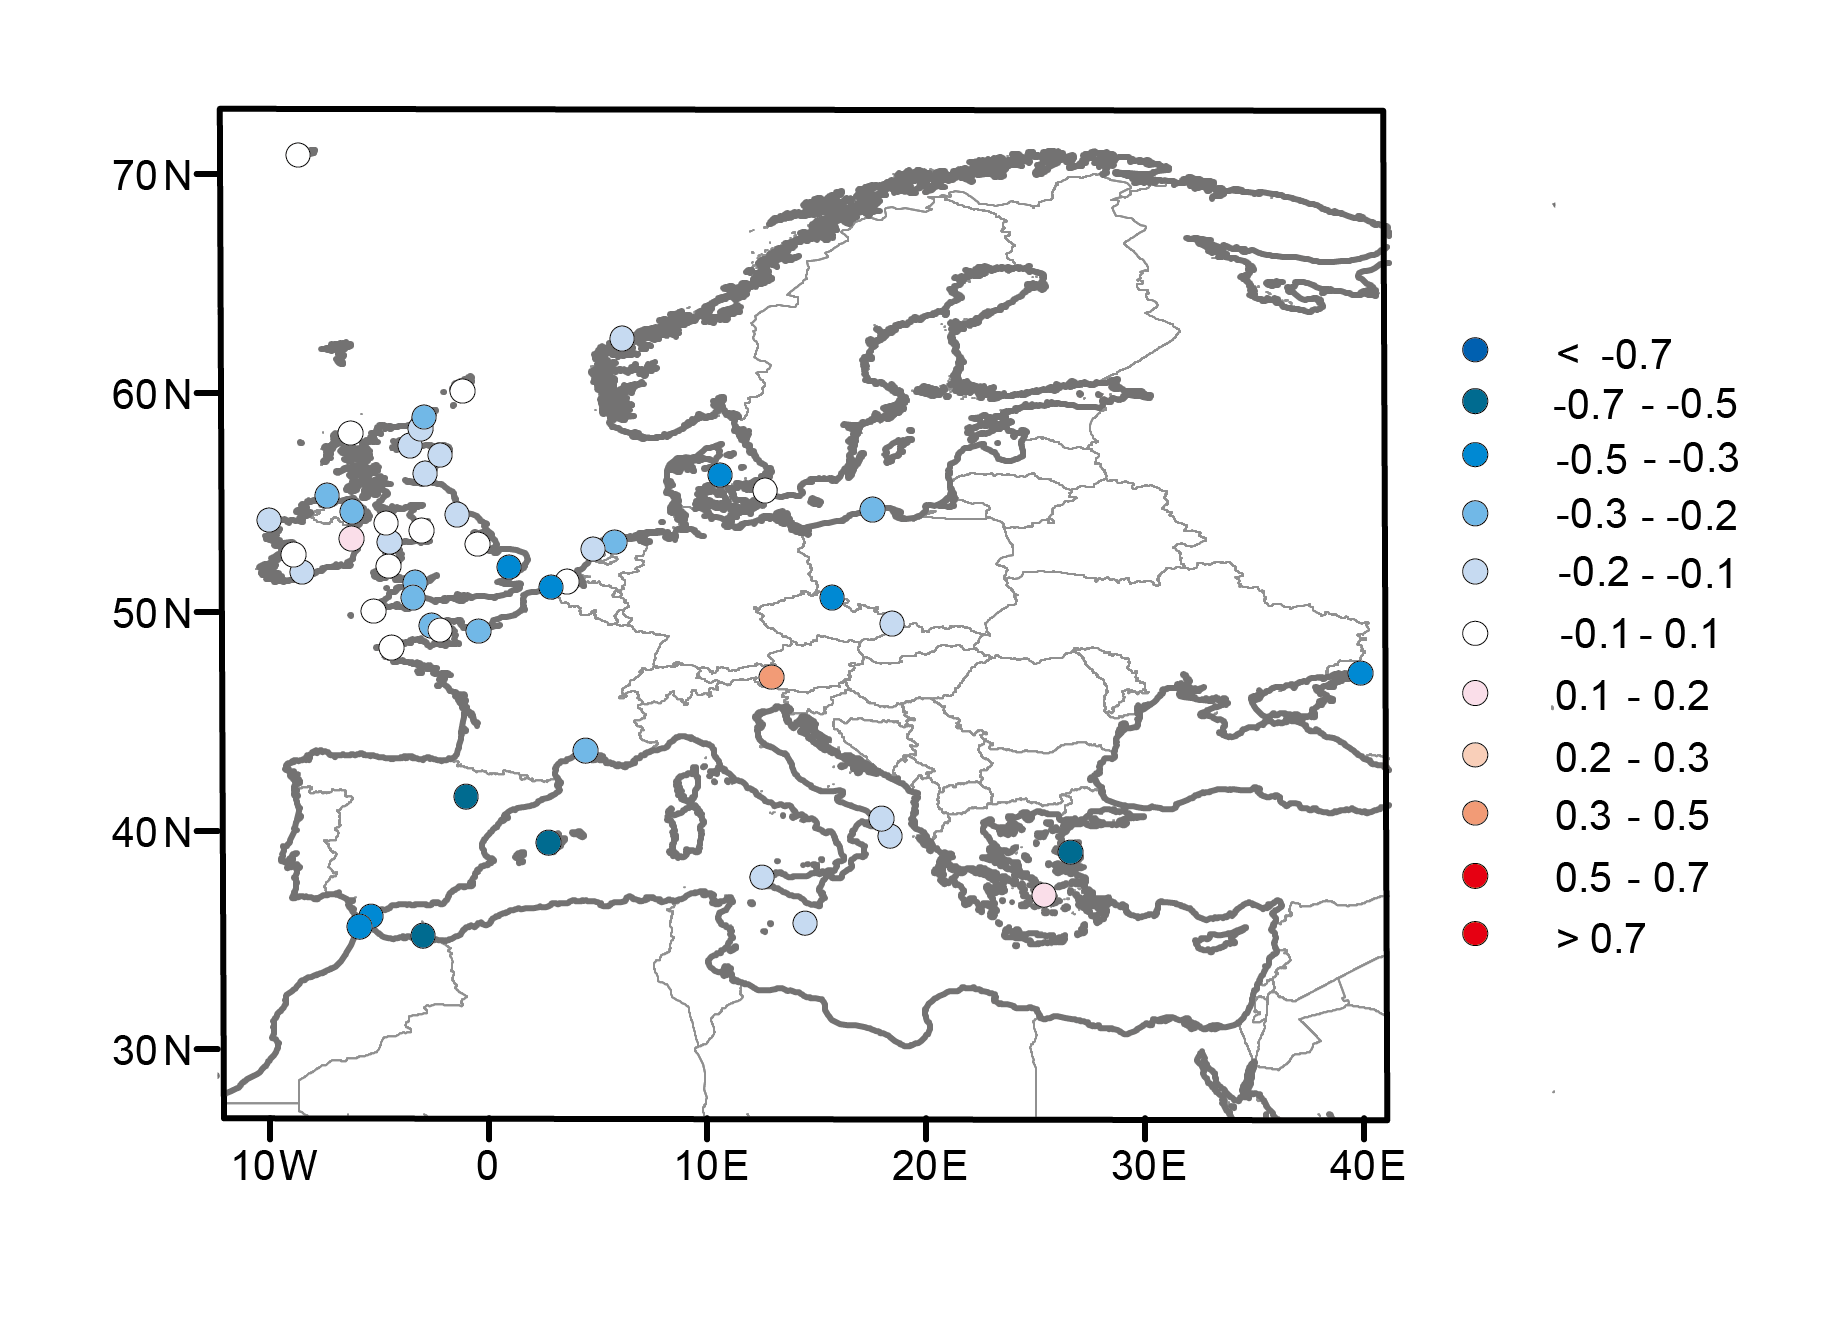
\includegraphics[width=0.95\textwidth]{欧洲大于3类风力站点风能密度变化}
    \bicaption{欧洲大于3类风力站点风能密度变化 (变化率)}{Change in wind power density at stations exceeding wind class 3 over North America (in $changing ~ rate$)}
    \label{fig:EUwindpowerchangeover3}
\end{figure}

\begin{figure}[!htbp]
    \centering
     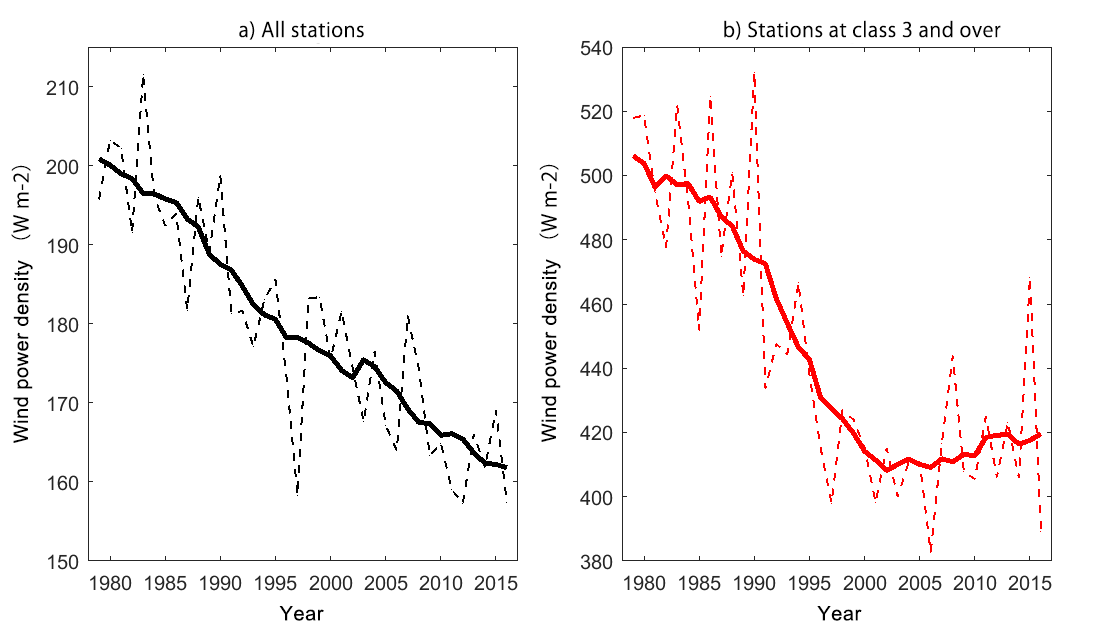
\includegraphics[width=0.9\textwidth]{欧洲风能密度演变}
    \bicaption{欧洲风能密度演变($ W ~ m^{-2}$)。与图 \ref{fig:NAwindpowerevolution}类似。}{Change in wind power density over Europe (in $ W ~ m^{-2}$). Same as Figure \ref{fig:NAwindpowerevolution}, but for Europe.}
    \label{fig:EUwindpowerevolution}
\end{figure}

亚洲531个站点风能密度变化中位数为-18.7\%,有49\%的站点风能密度下降超过20\%,21\%的站点下降超过50\%,同时有16\%的站点风能密度上升超过10\%,11\%的站点上升超过20\%。空间分布上,风能密度减小的站点大多分布在中国,日本的站点大部分风能密度增加或变化较小。由于中国是全球最大的风能市场,而相比之下日本的风能产业相对薄弱,装机容量仅为中国的1/70,因此以下重点分析中国的情况。中国有351个站点,风能密度变化中位数为-27\%,有47\%站点下降超过30\%,27\%的站点下降超过50\%,仅有9\%站点增加超过10\%,6\%站点增加超过20\%。风能密度减小较明显的地区是东北,新疆北部,云南南部,山东半岛和长江下游地区(图 \ref{fig:ASwindpowerchange})。中国超过3类风力的站点有16个,主要分布在东部沿海,新疆、内蒙古、甘肃、安徽和湖南也有分布。所有站点风能密度都出现了下降,中位数为-46\%,有一半的站点风能密度下降超过50\%,25\%站点下降超过70\%(图 \ref{fig:CHNwindpowerchangeover3})。中国站点中位数风能密度在1979年为50 $W ~ m^{-2}$左右,1979-1989年经历了一轮6 $W ~ m^{-2}$每十年的下降,在1989-1999年间稳定在44 $W ~ m^{-2}$附近,1999年之后又持续下降,趋势为5 $W ~ m^{-2}$,最终降到36 $W ~ m^{-2}$。而大于3类风力站电在1979-2016年期间持续下降,由500 $W ~ m^{-2}$下降到280 $W ~ m^{-2}$,趋势达到58 $W ~ m^{-2}$每十年(图 \ref{fig:CHNwindpowerevolution})。

\begin{figure}[!htbp]
    \centering
     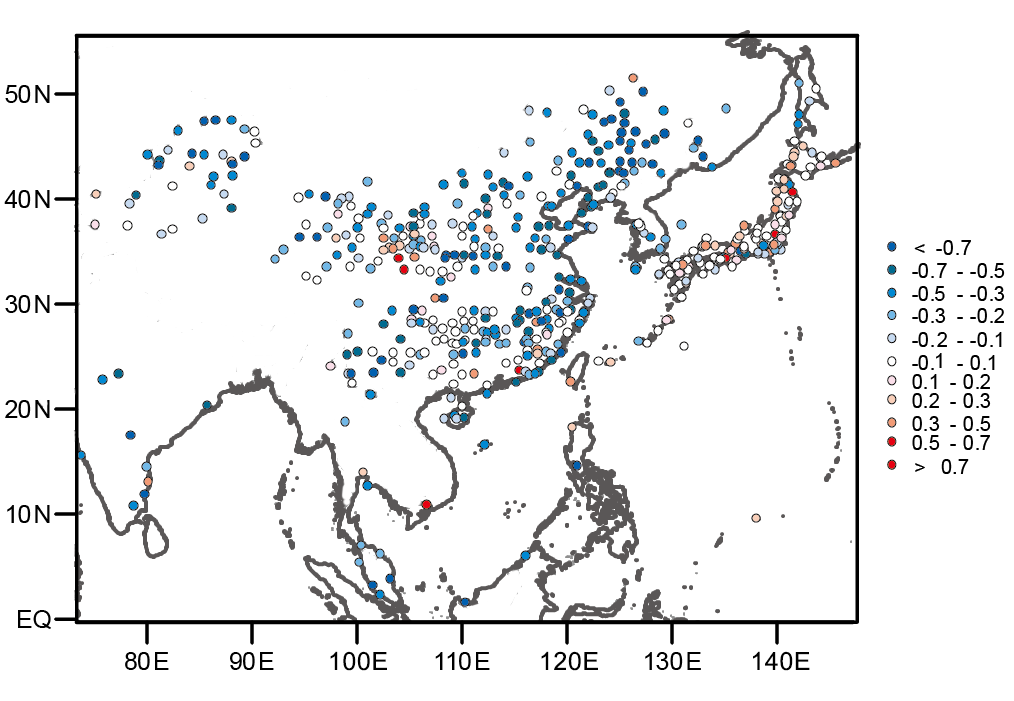
\includegraphics[width=0.95\textwidth]{亚洲风能密度变化}
    \bicaption{亚洲风能密度变化(变化率)}{Change in wind power density over Asia (in $changing ~ rate$)}
    \label{fig:ASwindpowerchange}
\end{figure}

\begin{figure}[!htbp]
    \centering
     \includegraphics[width=0.8\textwidth]{中国大于3类风力站点风能密度变化}
    \bicaption{中国大于3类风力站点风能密度变化 (变化率)}{Change in wind power density at stations exceeding wind class 3 over China (in $changing ~ rate$)}
    \label{fig:CHNwindpowerchangeover3}
\end{figure}

\begin{figure}[!htbp]
    \centering
     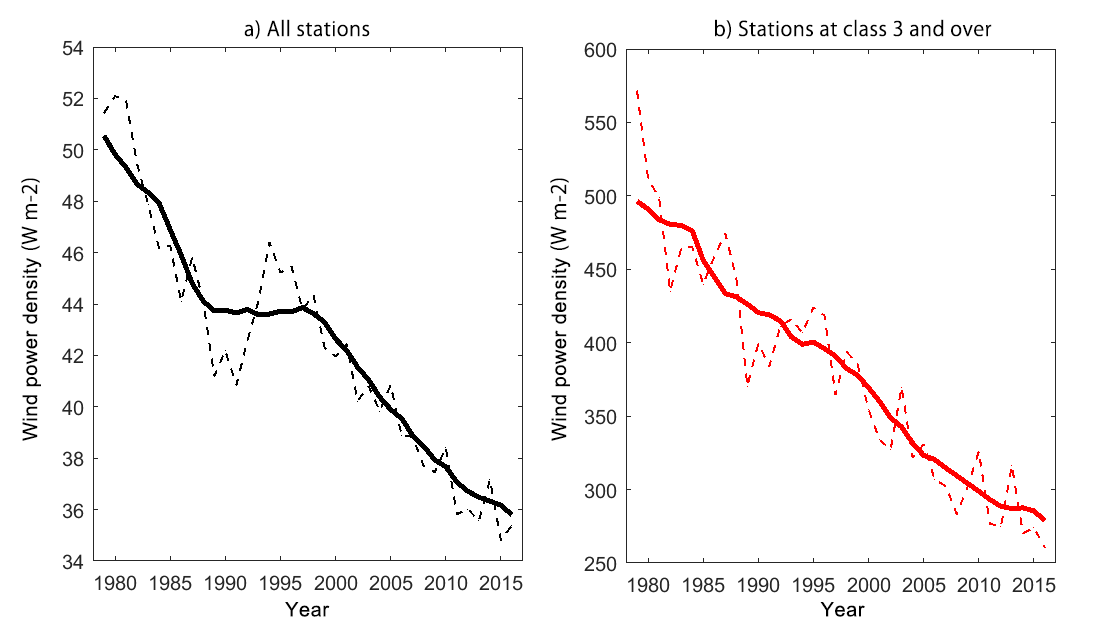
\includegraphics[width=0.9\textwidth]{中国风能密度演变}
    \bicaption{中国风能密度演变($ W ~ m^{-2}$)。与图 \ref{fig:NAwindpowerevolution}类似。}{Change in wind power density over China (in $ W ~ m^{-2}$). Same as Figure \ref{fig:NAwindpowerevolution}, but for China.}
    \label{fig:CHNwindpowerevolution}
\end{figure}

\section{风能资源长期变化模拟的不确定性}

由本章之前的分析可以得到,平均风速变化是风能密度长期变化的主导因素,因而本节对于风能密度长期变化模拟能力的分析将着重于评估模式对平均风速变化的模拟能力。将34个全球气候模式地表风速数据差值到NECI-CMDC站点位置,得到在1979-2005年间,14个模式的中位数风速与观测较为一致(差别小于0.17 $m ~ s^{-1}$,为观测的5\%),有6个模式与观测差别较大(大于0.7 $m ~ s^{-1}$,为观测的20\%):MIROC4h、CSIRO-Mk3.6.0、BCC-CSM1.1、BNU-ESM、BCC-CSM1.1(m) 和 CanESM2,其中CSIRO-Mk3.6.0地表风速高度为2 $m$。在此后风速长期变化的分析中将剔除掉这6个模式。在剩余的28个模式中,由18个表现出了风速下降,10个表现出了上升。三个风速下降最快的模式为MIROC5、HadGEM2-ES、MIROC-ESM-CHEM,风速趋势分别为-0.027、-0.014、-0.01 $m ~ s^{-1}$每十年,而观测风速趋势为0.095 $m ~ s^{-1}$每十年。因此,即使在风速下降最快的三个模式中,风速下降速度也远不及观测,下降最快的MIROC5趋势只有观测的30\%(表 \ref{tab:GCMoutputs},图 \ref{fig:GCMwind})。因此,CMIP5在地表风速长期趋势模拟上存在欠缺,因而对风能长期历史变化的模拟的不确定性较大。此前有研究表明,CMIP3同样不能很好模拟近几十年来风速长期趋势\citep{zongci2009evaluation},此现象值得风能研究者重视。

\begin{table}[!htbp]
    \bicaption{全球气候模式历史风速模拟结果 (1979-2005)}{Historical simulation of global climate models (1979-2005)}
    \label{tab:GCMoutputs}
    \centering
    \small% fontsize
    \setlength{\tabcolsep}{5 pt}% column separation
    \renewcommand{\arraystretch}{1.0}%row space 
    \begin{tabular}{lccc}
        \hline
         模式名称  $^{*}$& 模拟高度($m$) & 中位数风速($m ~ s^{-1}$) & 中位数趋势($m ~ s^{-1}$每十年) $^{**}$\\
        %\cline{2-9}% partial hline from column i to column j
        \hline
        观测 & 10 & 3.40 & -95 \\
        MIROC5 & 10 & 3.51 & -27 \\
        HadGEM2-ES & 10 & 2.91 & -14 \\
        MIROC-ESM-CHEM & 10 & 3.36 & -10\\
        MIROC-ESM & 10 & 3.30 & -9.3 \\
        GISS-E2-H & 10 & 3.20 & -9.0 \\
        \textbf{CSIRO-Mk3.6.0} & 2 & 2.02 & -8.6 \\
        CMCC-CMS & 10 & 3.56 & -8.6 \\
        CMCC-CM & 10 & 3.52 & -8.1 \\
        GISS-E2-R-CC & 10 & 3.34 & -7.9 \\
        \textbf{BNU-ESM} & 10 & 4.39 & -7.3 \\
        ACCESS1.3 & 10 & 3.32 & -6.4 \\
        GISS-E2-H-CC & 10 & 3.18 & -6.1 \\
        IPSL-CM5B-LR & 10 & 3.48 & -5.8 \\
        IPSL-CM5A-MR & 10 & 3.30 & -5.7 \\
        HadGEM2-AO & 10 & 2.95 & -5.1 \\
        GFDL-ESM2G & 10 & 3.31 & -4.8 \\
        GISS-E2-R & 10 & 3.35 & -4.6 \\
        HadCM3 & 10 & 3.87 & -3.7 \\
        \textbf{MIROC4h} & 10 & 2.70 & -1.6 \\
        ACCESS1.0 & 10 & 2.99 &  -1.2 \\
        MPI-ESM-MR & 10 & 3.91 & 1.7 \\
        \textbf{CanESM2} & 10 & 4.98 & 2.8 \\
        GFDL-ESM2M & 10 & 3.16 & 3.0 \\    
        GFDL-CM3 & 10 & 3.34 & 3.3 \\
        HadGEM2-CC & 10 & 2.91 & 3.4 \\
        \textbf{BCC-CSM1.1(m)} & 10 & 4.39 & 5.7 \\
        CMCC-CESM & 10 & 3.65 & 5.9 \\
        INM-CM4 & 10 & 3.61 & 8.3 \\
        IPSL-CM5A-LR & 10 & 3.27 & 10 \\
        \hline
	\end{tabular}
\end{table}
\begin{table}[!t]
    \ContinuedFloat% continue splited float
    \bicaption{续表。}{Continued table.}
    \label{tab:descriptionGCM2}
    \centering
    \small% fontsize
    \setlength{\tabcolsep}{27 pt}% column separation
    \renewcommand{\arraystretch}{1.0}%row space  
     \begin{tabular}{llll}
        \hline 
        \textbf{BCC-CSM1.1} & 10 & 4.92 & 12 \\
        MRI-CGCM3 & 10 & 3.27 & 12 \\
        MPI-ESM-P & 10 & 3.84 & 13 \\
        FGOALS-s2 & 10 & 3.84 & 16 \\
        MPI-ESM-LR & 10 & 3.94 & 20 \\
        \hline
      \end{tabular}
      
      \vspace*{3ex}  
      
    \begin{minipage}{0.8\textwidth}% choose width suitably
    注:$^*$ 加粗的模式平均风速偏差大于20\%。\\ 
    $^{**}$ 为了方便展示,中位数趋势结果已乘以$10^3$。
    \end{minipage}
\end{table}

\begin{figure}[!b]
    \centering
     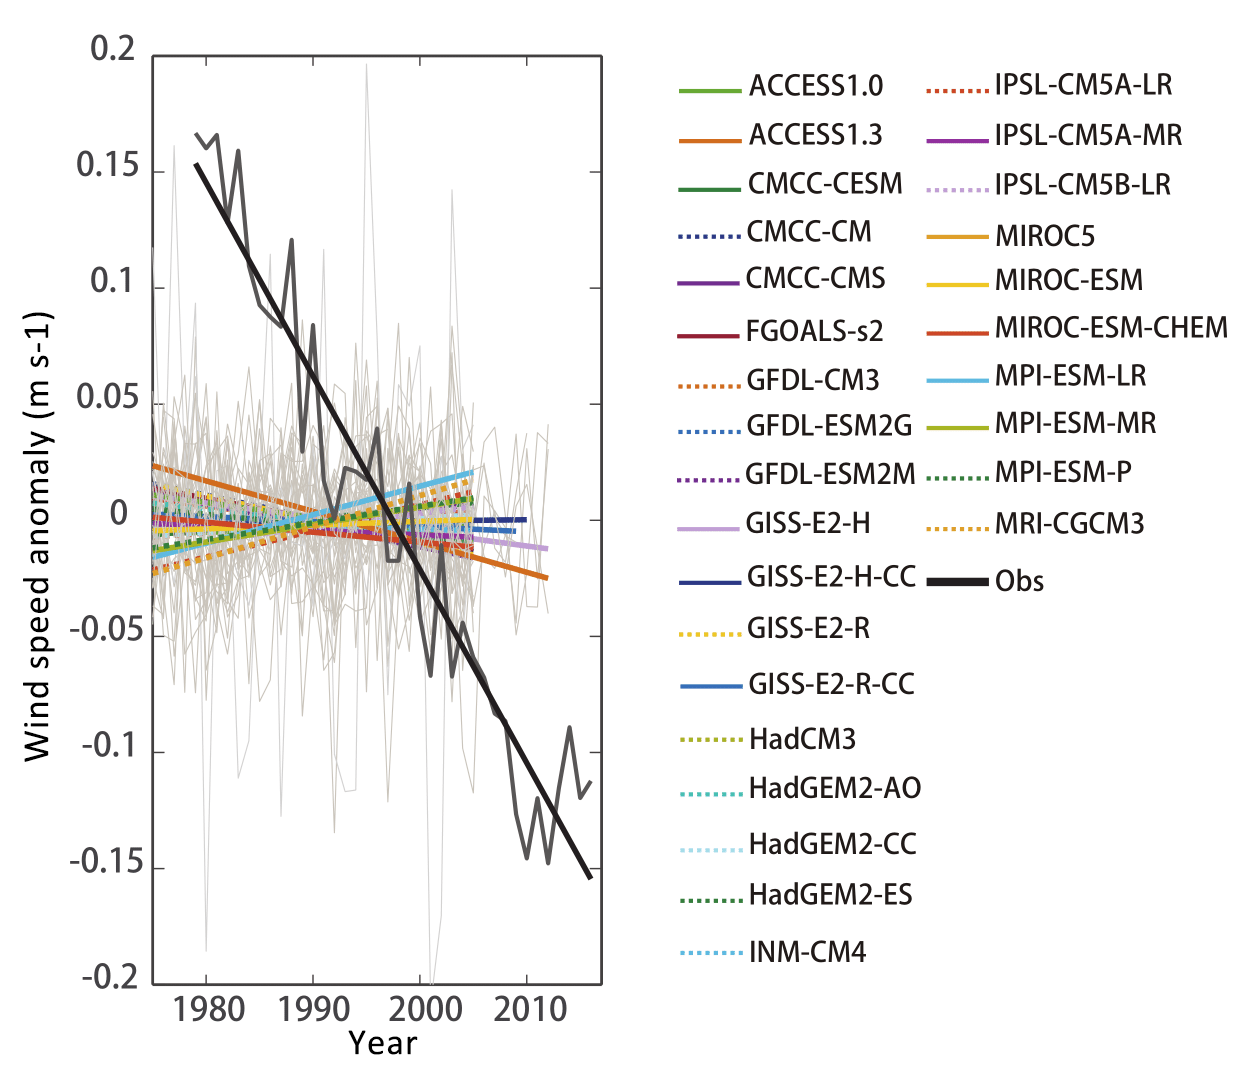
\includegraphics[width=0.9\textwidth]{北半球风速趋势模拟}
    \bicaption{全球气候模式模拟的北半球风速趋势。彩色线为模式结果,黑色线为观测结果。}{Wind speed trends over the Northern Hemisphere simulated by global climate models. Coloured lines are model outputs, black line is observation.}
    \label{fig:GCMwind}
\end{figure}

\section{本章小结}

本章评估了北半球近几十年来平均风能资源状况,分析了地表风速长期变化尤其是普遍减小的现象对于风能资源的影响,最后评估了全球气候模式对于风能历史长期变化的模拟能力,得到以下结论:

\begin{enumerate}

\item 风能资源北美洲和欧洲相对丰富,亚洲相对缺乏。北美洲风能资源丰富的地区集中在中部地带,欧洲主要集中在北海沿岸,亚洲主要集中在太平洋沿岸地区。风电场的分布主要集中在风能资源丰富地区,但也受到经济发展水平、社会观念、政策等因素等影响。

\item 受到地表风速普遍下降的影响,风能资源也经历了明显减少的过程,2012-2016年相对1979-1983年减小了14.8\%,亚洲风能资源减少最明显,欧洲次之,北美洲减少最慢,分别为-18.7\%、-15.2\%和-12.2\%。北美洲、欧洲和亚洲主要的风能市场中国大于3类风力站点风能资源下降速度都超过所在区域整体水平,分别为-16.7\%、-18\%和-46\%。

\item 风能资源的预估严重依赖全球气候模式,然而CMIP5全球气候模式模拟风能资源长期历史变化存在较大缺陷,因而使用其作为风能未来预估的工具有较大不确定性。

\end{enumerate}

